\documentclass{article}

\usepackage{style,xcolor}

% Sub-preambles
% https://github.com/MartinScharrer/standalone

% Encodings
\usepackage{amsmath,amssymb,gensymb,textcomp}
\usepackage{courier} %% Sets font for listing as Courier.
\usepackage{listings, xcolor}
% Better tables
% Wide tables go to https://tex.stackexchange.com/q/332902
\usepackage{array,multicol,multirow,siunitx,tabularx}
\usepackage{tabularray}

% Better enum
\usepackage{enumitem}

% Graphics
\usepackage{caption,float}

%lastpage
\usepackage{lastpage}

% Allow setting >max< width of figure
% Remove if unneeded
\usepackage[export]{adjustbox} % 'export' allows adjustbox keys in \includegraphics
\usepackage{mwe}

% Custom commands
% Remove if unneeded
\newcommand*\mean[1]{\bar{#1}}

\ocorso
\oreporttype{}
\title{ \emph{Ratatouille23}}
\reportlayout%

\numberwithin{equation}{section}
\numberwithin{figure}{section}

\begin{document}

\coverpage%

\section*{Gruppo INGSW2223\_N\_04}
\begin{center}
  \begin{tblr}{hlines = {0.9pt}, vlines = {0.9pt}, row{1} = {marroneApp!60}, colspec = {X[c]X[c]X[c]}, width = \textwidth}
        \textbf{No.} & \textbf{Nome e Cognome} & \textbf{Matricola} \\
        1            & Luigi Vessella          & N86003354\\
        2            & Matteo Marino           & N86003963\\
        3            & Biagio Speranza         & N86002964\\
  \end{tblr}
\end{center}

\newpage
\tableofcontents
\newpage
\section{Descrizione del progetto}
    {\large 
        Ratatouille23 è un sistema finalizzato al supporto alla gestione e all’operatività di attività di
        ristorazione. Il sistema consiste in un’applicazione performante e affidabile, attraverso cui gli utenti
        possono fruire delle funzionalità del sistema in modo intuitivo, rapido e piacevole. 
        La nostra visione della richiesta prevede lo sviluppo di un'applicazione mobile su sistema operativo Android che offrirà agli utilizzatori i seguenti servizi: 
    }
    
    \begin{itemize}
        \item  \emph{ I proprietari (o amministratori) potranno creare account per i dipendenti}
        \item  \emph{I proprietari saranno in grado di gestire uno o più ristoranti}
        \item  \emph{Si avrà la possibilità di visualizzare e/o modificare il menu}
        \item  \emph{I dipendenti (camerieri) saranno in grado di prendere e inoltrare le ordinazioni in cucina}
        \item  \emph{Gli addetti alla cucina potranno avvisare i camerieri nel momento in cui è pronta un'ordinazione}
        \item  \emph{Tutti potranno visionare lo storico delle ordinazioni con i dettagli}
    \end{itemize} 
    
    \begin{flushleft}
      {\large Ovviamente, il tipo di funzionalità messo a disposizione dall'applicativo sarà cambiato
        dinamicamente a seconda di chi si logga. 
        Gli amministratori e/o supervisori saranno inoltre dotati di tablet con a bordo l'OS di Google Android per
        una migliore fruizione della loro dashboard.}

      \vspace{1cm}

    {\large I dipendenti quali camerieri, operatori di cucina, capisala, saranno dotati di smartphone aziendali sempre con OS Android correttamente configurati per un'ottimale fruizione dell'applicazione.}
      \vspace{1cm}

    {\large \textbf{Tutti i dispositivi dovranno essere in grado di accedere a internet, preferibilmente per tutta la durata del servizio. Il funzionamento del server è invece garantito da servizi allo stato dell'arte quali Microsoft Azure.}}
    \end{flushleft}
    
    \subsection{Premessa e presentazione}
    \begin{figure}[H]
        \centering
        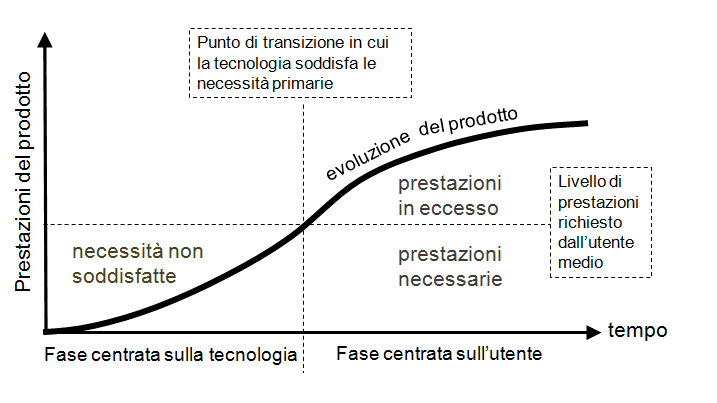
\includegraphics[scale=0.5]{assets/immagini varie/D.Norman grafico.png}
        \caption{\textbf{Grafico}: Evoluzione dei prodotti high-tech secondo D.Norman}\label{fig:Figure_D.Norman}
    \end{figure}

    \begin{flushleft}
        
        Con questo piccolo preambolo vogliamo richiamare l'attenzione sul diagramma di evoluzione dei prodotti software di D.Norman, il quale mostra il ciclo di vita che solitamente questo tipo di prodotto ha.
        All'inizio avremo un'app più incentrata sulle tecnologie implementate e/o da implementare per  "cercare " di raggiungere ciò che l'utente medio richiede dall'applicativo. Successivamente si otterrà il punto di pareggio in cui si soddisfano
        i bisogni dell'utente tipico, e ciò potrebbe essere considerato un buon punto di equilibrio del sistema.
        In fine, sempre ammesso che l'app sia sopravvissuta al mercato durante questo ciclo, ci può essere una fase finale con una condizione
        di iperfunzionalità, dove si cercherà via via di soddisfarre le esigenze di una platea di utenti più ampia. Nel caso della nostra applicazione Ratatouille23 descritta in questo documento, pensiamo di distribuire un prodotto nella sua 
        fase di equilibrio (vedere grafico) che certamente soddisfa le esigenze degli attori utilizzatori descritti nei punti successivi, ma che allo stesso tempo può essere facilmente aggiornata e migliorata qualora dovessero aggiungersi nuovi target d'utenti o cambiare
        gli esistenti.
    \end{flushleft}
 
    \section{Documento dei requisiti software}
    \subsection{Requisiti Funzionali}
        \begin{flushleft}  
            {\large
                Vengono qui presentati i requisiti funzionali dell'applicativo, ossia quei servizi che l'app  deve offrire agli utenti:
            } 
        \end{flushleft}
        
        \subsubsection{Admin}
        

        \begin{center}
          % Admin 1
          \begin{tblr}{hlines = {0.9pt}, vlines = {0.9pt}, row{1} = {marroneApp!60}, colspec = {X[c]X[l]}, width = \textwidth}
                  \textbf{ID}         & Admin\_1                             \\
                  \textbf{Nome}       & Registrazione account amministratore \\
                  \textbf{Descrizione} & {Il sistema permette ad un amministratore non registrato di registrarsi alla\\ piattaforma utilizzando: \textit{nome}, \textit{cognome}, \textit{email}, \textit{codice fiscale}, \textit{P.IVA} e \textit{password}}
          \end{tblr}

          \vspace{1cm}

          % Admin 2
          \begin{tblr}{hlines = {0.9pt}, vlines = {0.9pt}, row{1} = {marroneApp!60}, colspec = {X[c]X[l]}, width = \textwidth}
                  \textbf{ID}         & Admin\_2                             \\
                  \textbf{Nome}       & Modifica account amministratore \\
                  \textbf{Descrizione} & {Il sistema permette ad un amministratore loggato di modifcare i campi del proprio account}
          \end{tblr}

          \vspace{1cm}

          % Admin 3
          \begin{tblr}{hlines = {0.9pt}, vlines = {0.9pt}, row{1} = {marroneApp!60}, colspec = {X[c]X[l]}, width = \textwidth}
                  \textbf{ID}         & Admin\_3                             \\
                  \textbf{Nome}       & Registrazione dei dipendenti \\
                  \textbf{Descrizione} & {Il sistema permette ad un amministratore di creare utenze per i dipendenti non registrati del ristorante,\\ specificandone \textit{nome}, \textit{cognome}, \textit{email} e \textit{ruolo}}
          \end{tblr}

          \vspace{1cm}

          % Admin 4
          \begin{tblr}{hlines = {0.9pt}, vlines = {0.9pt}, row{1} = {marroneApp!60}, colspec = {X[c]X[l]}, width = \textwidth}
                  \textbf{ID}          & Admin\_4                             \\
                  \textbf{Nome}        & Modificare/Eliminare account dipendenti  \\
                  \textbf{Descrizione} & {Il sistema permette ad un amministratore loggato di modificare gli account dei propri dipendenti.}
          \end{tblr}

          \vspace{1cm}

          % Admin 5
          \begin{tblr}{hlines = {0.9pt}, vlines = {0.9pt}, row{1} = {marroneApp!60}, colspec = {X[c]X[l]}, width = \textwidth}
                  \textbf{ID}          & Admin\_5                             \\
                  \textbf{Nome}        & Aggiungere personale della cucina  \\
                  \textbf{Descrizione} & {Il sistema permette ad un amministratore loggato di aggiungere al proprio ristorante il personale della cucina.}
          \end{tblr}

          \vspace{1cm}

          % Admin 6
          \begin{tblr}{hlines = {0.9pt}, vlines = {0.9pt}, row{1} = {marroneApp!60}, colspec = {X[c]X[l]}, width = \textwidth}
                  \textbf{ID}          & Admin\_6                             \\
                  \textbf{Nome}        & Aggiunta dei Ristoranti  \\
                  \textbf{Descrizione} & {Il sistema permette ad un amministratore di poter aggiungere le proprie attività di ristorazione (CAMPI DA DEFINIRE).}
          \end{tblr}

          \vspace{1cm}

          % Admin 7
          \begin{tblr}{hlines = {0.9pt}, vlines = {0.9pt}, row{1} = {marroneApp!60}, colspec = {X[c]X[l]}, width = \textwidth}
                  \textbf{ID}          & Admin\_7                             \\
                  \textbf{Nome}        &  Modifica/Eliminazione dei Ristoranti  \\
                  \textbf{Descrizione} & {Il sistema permette ad un amministratore di poter modificare ed eliminare le proprie attività di ristorazione del sistema.}
          \end{tblr}

          \vspace{1cm}

          % Admin 8
          \begin{tblr}{hlines = {0.9pt}, vlines = {0.9pt}, row{1} = {marroneApp!60}, colspec = {X[c]X[l]}, width = \textwidth}
                  \textbf{ID}          & Admin\_8                             \\
                  \textbf{Nome}        &  Modifica dati dei Dipendenti  \\
                  \textbf{Descrizione} & {Il sistema permette ad un amministratore loggato di poter cambiare i dati personali dei dipendenti (nome, cognome, email, luogo).}
          \end{tblr}

          \vspace{1cm}

          % Admin 9
          \begin{tblr}{hlines = {0.9pt}, vlines = {0.9pt}, row{1} = {marroneApp!60}, colspec = {X[c]X[l]}, width = \textwidth}
                  \textbf{ID}          & Admin\_9                             \\
                  \textbf{Nome}        &  Aggiungere/Modificare elementi nel menù  \\
                  \textbf{Descrizione} & {Il sistema permette ad un amministratore o supervisore dell'attività di ristorazione di aggiungere/modificare elementi nel menù dell'attività. Ogni elemento dovrà avere i seguenti campi:\\ Nome, Costo, Descrizione, Elenco di Allergeni, Categoria/e}
          \end{tblr}

          \vspace{1cm}

          % Admin 10
          \begin{tblr}{hlines = {0.9pt}, vlines = {0.9pt}, row{1} = {marroneApp!60}, colspec = {X[c]X[l]}, width = \textwidth}
                  \textbf{ID}          & Admin\_10                             \\
                  \textbf{Nome}        &  Modifica dati personali\\
                  \textbf{Descrizione} & {Il sistema permette ad un amministratore loggato di poter cambiare i propri dati  personali.}
          \end{tblr}

          \vspace{1cm}

          % Admin 12
          \begin{tblr}{hlines = {0.9pt}, vlines = {0.9pt}, row{1} = {marroneApp!60}, colspec = {X[c]X[l]}, width = \textwidth}
                  \textbf{ID}          & Admin\_12                             \\
                  \textbf{Nome}        &  Tradurre il menu           \\
                  \textbf{Descrizione} & {Il sistema permette ad un Amministratore di poter tradurre gli elementi del proprio menù in un altra lingua}
          \end{tblr}

          \vspace{1cm}

          % Admin 13
          \begin{tblr}{hlines = {0.9pt}, vlines = {0.9pt}, row{1} = {marroneApp!60}, colspec = {X[c]X[l]}, width = \textwidth}
                  \textbf{ID}          & Admin\_13                             \\
                  \textbf{Nome}        &  Visualizza statistiche personale della cucina\\
                  \textbf{Descrizione} & {Il sistema permette ad un Amministratore di visualizzare, grazie anche all'ausilio di grafici interattivi, informazioni sull'operato degli addetti alla cucina}
          \end{tblr}

          \vspace{1cm}

          % Admin 14
          \begin{tblr}{hlines = {0.9pt}, vlines = {0.9pt}, row{1} = {marroneApp!60}, colspec = {X[c]X[l]}, width = \textwidth}
                  \textbf{ID}          & Admin\_14                             \\
                  \textbf{Nome}        & Modifica menu \\
                  \textbf{Descrizione} & {Il sistema permette ad un Amministratore di poter aggiornare (aggiungere, modificare ed eliminare elementi) il menu del ristorante}
          \end{tblr}
        \end{center}

        \subsubsection{Cameriere}
        \begin{center}

          % Waiter 1
          \begin{tblr}{hlines = {0.9pt}, vlines = {0.9pt}, row{1} = {marroneApp!60}, colspec = {X[c]X[l]}, width = \textwidth}
                  \textbf{ID}          & Waiter\_1                             \\
                  \textbf{Nome}        & Prendere le ordinazioni \\
                  \textbf{Descrizione} & {Il sistema permette ai camerieri di prendere ordinazioni ai tavoli, inoltrandole alla cucina.}
          \end{tblr}

          \vspace{1cm}

          % Waiter 2
          \begin{tblr}{hlines = {0.9pt}, vlines = {0.9pt}, row{1} = {marroneApp!60}, colspec = {X[c]X[l]}, width = \textwidth}
                  \textbf{ID}          & Waiter\_2                             \\
                  \textbf{Nome}        & Gestione delle ordinazioni \\
                  \textbf{Descrizione} & {Il sistema permette ai camerieri di prendere ordinazioni ai tavoli, inoltrandole alla cucina.}
          \end{tblr}

          \vspace{1cm}

          % Waiter 3
          \begin{tblr}{hlines = {0.9pt}, vlines = {0.9pt}, row{1} = {marroneApp!60}, colspec = {X[c]X[l]}, width = \textwidth}
                  \textbf{ID}          & Waiter\_3                             \\
                  \textbf{Nome}        & Evasione degli ordini \\
                  \textbf{Descrizione} & {Il sistema permette a un Cameriere di marcare i singoli elementi di un ordine come conclusi, aggiornando gli addetti in cucina}
          \end{tblr}

          \vspace{1cm}

          % Waiter 4
          \begin{tblr}{hlines = {0.9pt}, vlines = {0.9pt}, row{1} = {marroneApp!60}, colspec = {X[c]X[l]}, width = \textwidth}
                  \textbf{ID}          & Waiter\_4                             \\
                  \textbf{Nome}        & Sollecitare la cucina \\
                  \textbf{Descrizione} & {Il sistema permette a un Cameriere di sollecitare la cucina nel caso in cui un ordine sia da troppo tempo in preparazione }
          \end{tblr}

        \end{center}
        
        \subsubsection{Cucina}

        \begin{center}
          % Kitchen 1
          \begin{tblr}{hlines = {0.9pt}, vlines = {0.9pt}, row{1} = {marroneApp!60}, colspec = {X[c]X[l]}, width = \textwidth}
                  \textbf{ID}          & Kitchen\_1                             \\
                  \textbf{Nome}        & Marcare gli ordini pronti \\
                  \textbf{Descrizione} & {Il sistema permette alla cucina di marcare gli ordini pronti alla "consegna", specificando lo chef che l'ha preparato}
          \end{tblr}

          \vspace{1cm}

          % Kitchen 2
          \begin{tblr}{hlines = {0.9pt}, vlines = {0.9pt}, row{1} = {marroneApp!60}, colspec = {X[c]X[l]}, width = \textwidth}
                  \textbf{ID}          & Kitchen\_2                             \\
                  \textbf{Nome}        & Sollecitare i camerieri \\
                  \textbf{Descrizione} & {Il sistema permette alla cucina di notificare i camerieri nel caso in cui un ordine sia pronto alla consegna da troppo tempo }
          \end{tblr}

        \end{center}

        \subsubsection{Supervisore}

        \begin{center}

          % Hypervisor 1 (Forse Supervisor (?))
          \begin{tblr}{hlines = {0.9pt}, vlines = {0.9pt}, row{1} = {marroneApp!60}, colspec = {X[c]X[l]}, width = \textwidth}
                  \textbf{ID}          & Hypervisor\_1                             \\
                  \textbf{Nome}        & Avvisare il personale \\
                  \textbf{Descrizione} & {Il sistema permette ad un supervisore ed un amministratore di inviare degli avvisi al personale}
          \end{tblr}

          \vspace{1cm}

          % Hypervisor 2 (Forse Supervisor (?))
          \begin{tblr}{hlines = {0.9pt}, vlines = {0.9pt}, row{1} = {marroneApp!60}, colspec = {X[c]X[l]}, width = \textwidth}
                  \textbf{ID}          & Hypervisor\_2                             \\
                  \textbf{Nome}        & Visualizzare stato ordini per tavolo\\
                  \textbf{Descrizione} & {Il sistema permette ad un Supervisore ed un Cameriere di visualizzare gli stati delle ordinazioni per ogni tavolo}
          \end{tblr}

          \vspace{1cm}

          % Hypervisor 3 (Forse Supervisor (?))
          \begin{tblr}{hlines = {0.9pt}, vlines = {0.9pt}, row{1} = {marroneApp!60}, colspec = {X[c]X[l]}, width = \textwidth}
                  \textbf{ID}          & Hypervisor\_3                             \\
                  \textbf{Nome}        & Visualizzare ordini in arrivo\\
                  \textbf{Descrizione} & {Il sistema permette ad un Supervisore e alla Cucina di visualizzare l'elenco di ordini in arrivo}
          \end{tblr}

          \vspace{1cm}

          % Hypervisor 4 (Forse Supervisor (?))
          \begin{tblr}{hlines = {0.9pt}, vlines = {0.9pt}, row{1} = {marroneApp!60}, colspec = {X[c]X[l]}, width = \textwidth}
                  \textbf{ID}          & Hypervisor\_4                             \\
                  \textbf{Nome}        & Visualizzare ordini in uscita\\
                  \textbf{Descrizione} & {Il sistema permette ad un Supervisore e alla Cucina di visualizzare l'elenco di ordini pronti all'uscita}
          \end{tblr}

          \vspace{1cm}

          % Hypervisor 5 (Forse Supervisor (?))
          \begin{tblr}{hlines = {0.9pt}, vlines = {0.9pt}, row{1} = {marroneApp!60}, colspec = {X[c]X[l]}, width = \textwidth}
                  \textbf{ID}          & Hypervisor\_5                             \\
                  \textbf{Nome}        & Visualizzare storico ordini\\
                  \textbf{Descrizione} & {Il sistema permette ad un Supervisore e alla Cucina di visualizzare lo storico degli ordini}
          \end{tblr}

          \vspace{1cm}
        \end{center}


        \subsubsection{Tutti}

        \begin{center}

          % All 1
          \begin{tblr}{hlines = {0.9pt}, vlines = {0.9pt}, row{1} = {marroneApp!60}, colspec = {X[c]X[l]}, width = \textwidth}
                  \textbf{ID}          & All\_1                             \\
                  \textbf{Nome}        & Recupero/Cambio Password\\
                  \textbf{Descrizione} & {Il sistema permette a tutti gli utenti registrati di poter recuperare la password e di poterla modificare}
          \end{tblr}

          \vspace{1cm}

          % All 2
          \begin{tblr}{hlines = {0.9pt}, vlines = {0.9pt}, row{1} = {marroneApp!60}, colspec = {X[c]X[l]}, width = \textwidth}
                  \textbf{ID}          & All\_2                             \\
                  \textbf{Nome}        & Login\\
                  \textbf{Descrizione} & {Il sistema permette a tutti gli utenti registrati di poter effettuare il login con Username e Password all'interno della piattaforma}
          \end{tblr}

          \vspace{1cm}

          % All 3
          \begin{tblr}{hlines = {0.9pt}, vlines = {0.9pt}, row{1} = {marroneApp!60}, colspec = {X[c]X[l]}, width = \textwidth}
                  \textbf{ID}          & All\_3                             \\
                  \textbf{Nome}        & Visualizzare un avviso o sollecitazione\\
                  \textbf{Descrizione} & {Il sistema permette a tutti gli utenti registrati pi poter visualizzare gli avvisi e le sollecitazioni ricevuti, marcandoli come visualizzati}
          \end{tblr}
        \end{center}

        \newpage

        \subsection{Requisiti Non Funzionali}
        \begin{flushleft} Vengono qui elencati i requisiti non funzionali dell'applicativo: \end{flushleft}

        \begin{center}
          % Unfunctional 1
          \begin{tblr}{hlines = {0.9pt}, vlines = {0.9pt}, row{1} = {marroneApp!60}, colspec = {X[c]X[l]}, width = \textwidth}
                  \textbf{ID}          & Unfunctional\_1                             \\
                  \textbf{Nome}        & Policy first password\\
                  \textbf{Descrizione} & {Il sistema richiede al primo accesso di un dipendente il cambio della password provvisoria in una password personale.}
          \end{tblr}

          \vspace{1cm}

          % Unfunctional 2
          \begin{tblr}{hlines = {0.9pt}, vlines = {0.9pt}, row{1} = {marroneApp!60}, colspec = {X[c]X[l]}, width = \textwidth}
                  \textbf{ID}          & Unfunctional\_2                             \\
                  \textbf{Nome}        & Verifica esistenza della mail\\
                  \textbf{Descrizione} & {Al fine di evitare registrazioni con e-mail fittizie, il sistema richiede l'autenticazione della mail mediante codice di verifica per poter procedere con il completamento della registrazione}
          \end{tblr}

          \vspace{1cm}

          % Unfunctional 3
          \begin{tblr}{hlines = {0.9pt}, vlines = {0.9pt}, row{1} = {marroneApp!60}, colspec = {X[c]X[l]}, width = \textwidth}
                  \textbf{ID}          & Unfunctional\_3                             \\
                  \textbf{Nome}        & Password Strength\\
                  \textbf{Descrizione} & {Al fine di evitare la creazione di password poco sicure, il sistema impone all'utente di utilizzare una password di almeno 8 caratteri che contenga numeri e caratteri speciali.}
          \end{tblr}

          \vspace{1cm}

          % Unfunctional 4
          \begin{tblr}{hlines = {0.9pt}, vlines = {0.9pt}, row{1} = {marroneApp!60}, colspec = {X[c]X[l]}, width = \textwidth}
                  \textbf{ID}          & Unfunctional\_4                             \\
                  \textbf{Nome}        & \textcolor{red}{TODO}\\
                  \textbf{Descrizione} & {Una P.IVA appartiene ad un solo amministratore.}
          \end{tblr}
        \end{center}

        \subsection{Requisiti di Dominio}

        \begin{center}
          % Domain 1
          \begin{tblr}{hlines = {0.9pt}, vlines = {0.9pt}, row{1} = {marroneApp!60}, colspec = {X[c]X[l]}, width = \textwidth}
                  \textbf{ID}          & Domain\_1                             \\
                  \textbf{Nome}        & GDPR\\
                  \textbf{Descrizione} & {Il sistema deve essere conforme alla normativa GDPR (Regolamento Generale  sulla Protezione dei Dati), per il trattamento dei dati personali e riguardante la privacy dell'utente}
          \end{tblr}
        \end{center}
    \subsection{Modellazione dei casi d'uso}

    \begin{flushleft}
        In questa sezione vengono riportati i Use-case diagram relativi al sistema, le tabelle di Cockburn e i Sequence diagram relativi alle funzionalità  \emph{\textbf{Aggiungi ristorante}},  \emph{\textbf{Aggiungi piatto}},  \emph{\textbf{Prendi ordinazione}},  \emph{\textbf{Visualizza avvisi}}.
    \end{flushleft}

    \subsubsection{Use-Case Diagram}
        \begin{flushleft}
            Qui viene riportato lo Use Case Diagram relativo all'applicazione, che per rendere la lettura più semplificata 
            è stato diviso in più sezioni.
        \end{flushleft}
        
        \begin{figure}[H]
            \centering
            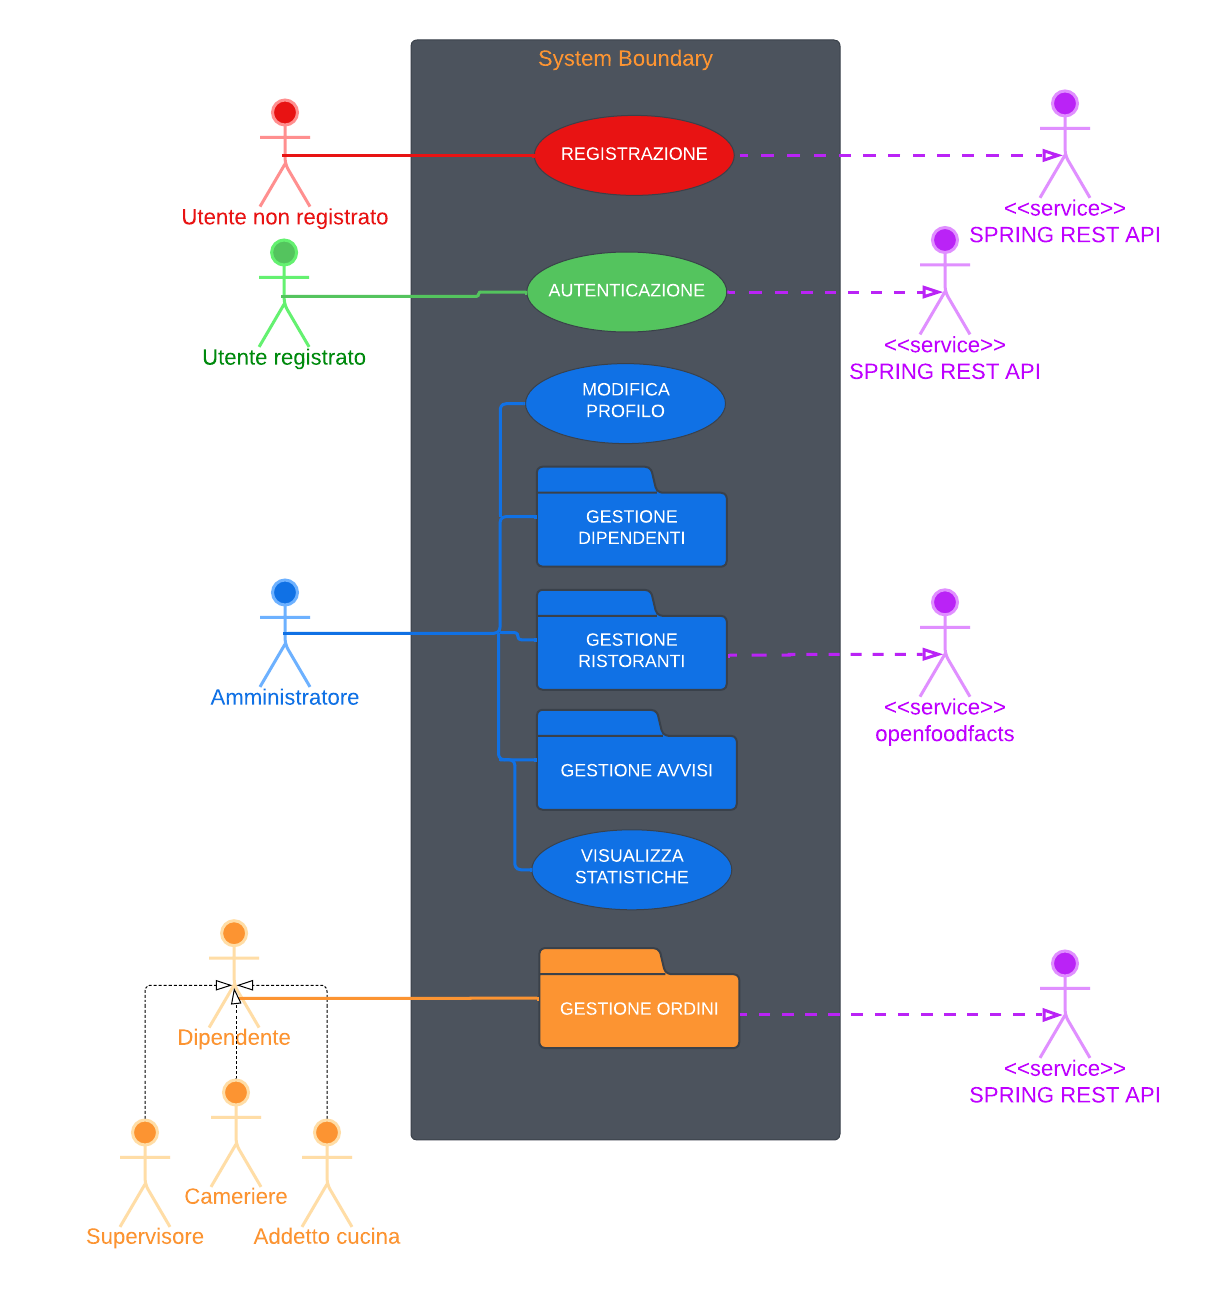
\includegraphics[width=0.8\textwidth]{assets/diagrammi/Use-Case/Use-Case Generale.png}
            \caption{Use Case dell'applicazione}
            \label{fig:ucdGenerale}
        \end{figure}
        
        \begin{figure}[H]
            \centering
            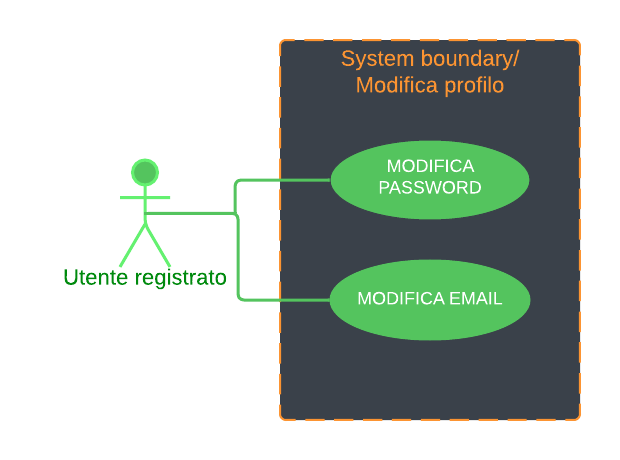
\includegraphics[width=0.8\textwidth]{assets/diagrammi/Use-Case/Modifica Profilo.png}
            \caption{Use Case relativo alla modifica del profilo}
            \label{fig:ucdModProfile}
        \end{figure}

        \begin{figure}[H]
            \centering
            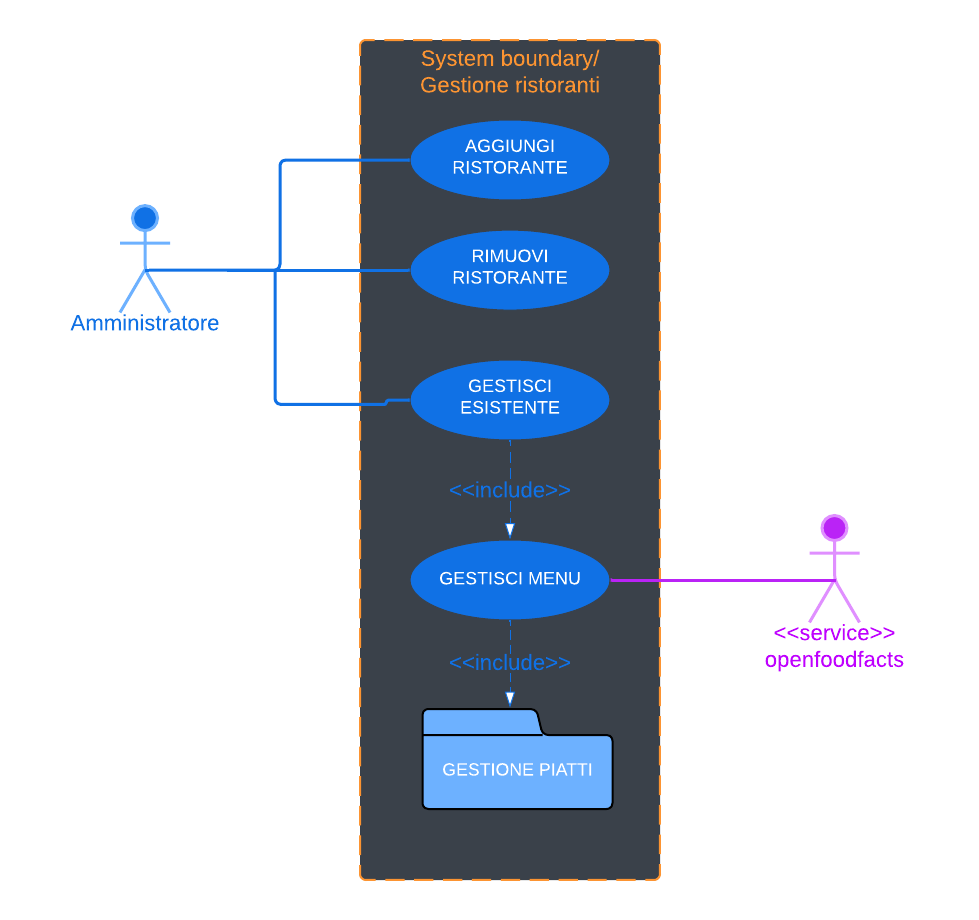
\includegraphics[width=0.8\textwidth]{assets/diagrammi/Use-Case/Gestione ristoranti.png}
            \caption{Use Case relativo alla gestione dei ristoranti}
            \label{fig:ucdResturantMgmt}
        \end{figure}

        \begin{figure}[H]
            \centering
            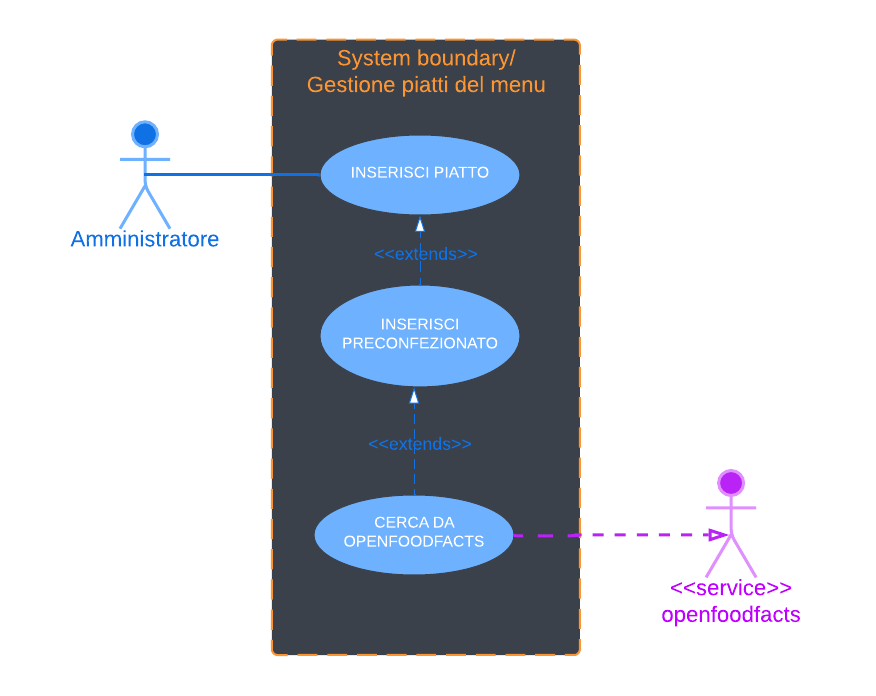
\includegraphics[width=0.8\textwidth]{assets/diagrammi/Use-Case/Gestione piatti.png}
            \caption{Use Case relativo alla gestione dei piatti del menù}
            \label{fig:ucdPlatesMgmt}
        \end{figure}

        \begin{figure}[H]
            \centering
            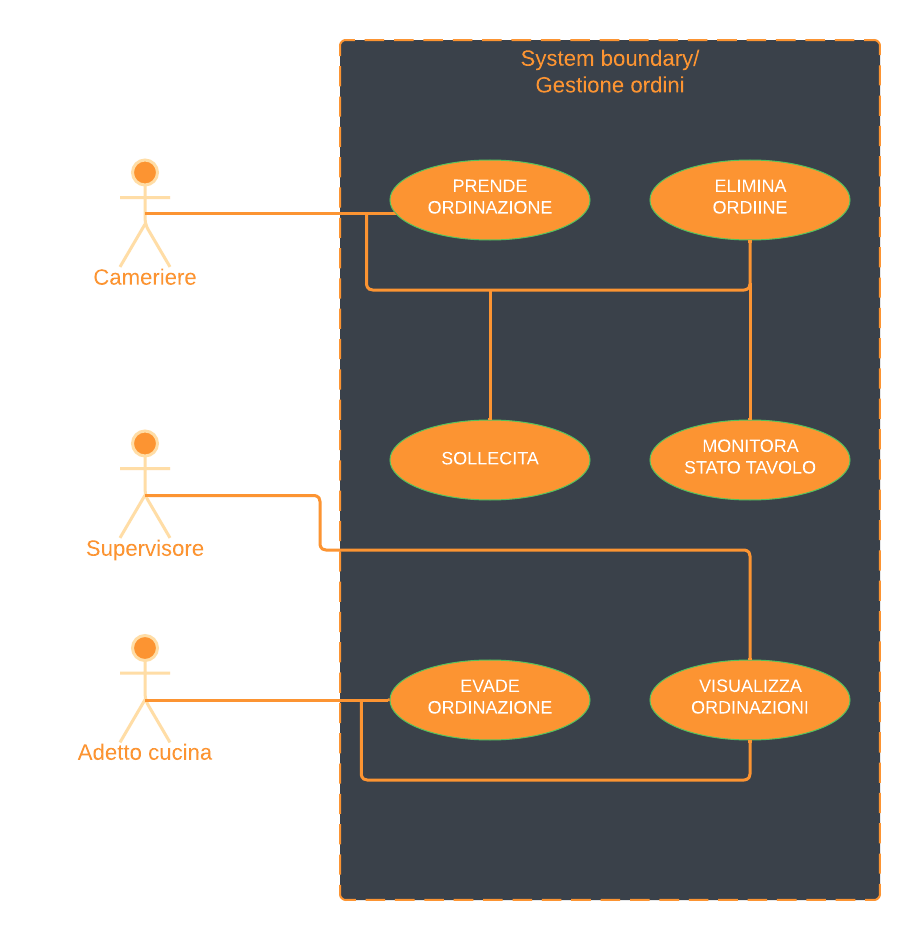
\includegraphics[width=0.7\textwidth]{assets/diagrammi/Use-Case/Gestione ordini.png}
            \caption{Use Case relativo alla gestione degli ordini}
            \label{fig:ucdOrderMgmt}
        \end{figure}
        
        \begin{figure}[H]
            \centering
            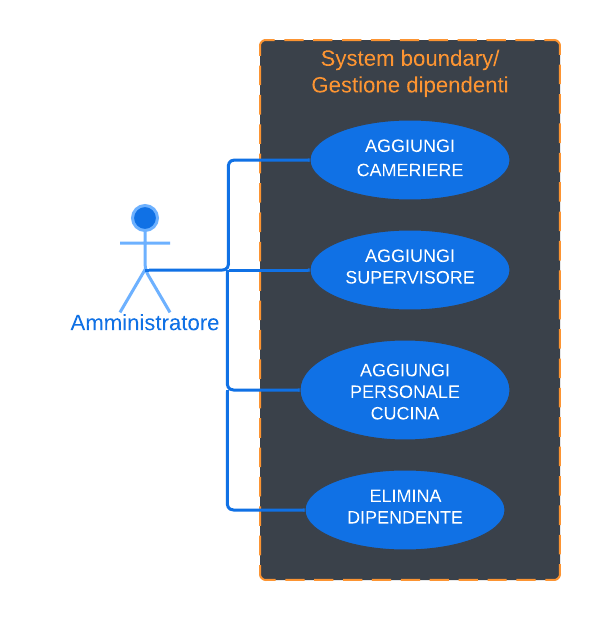
\includegraphics[width=0.6\textwidth]{assets/diagrammi/Use-Case/Gestione dipendenti.png}
            \caption{Use Case relativo alla gestione dei dipendenti}
            \label{fig:ucdWorkersMgmt}
        \end{figure}

        \begin{figure}[H]
            \centering
            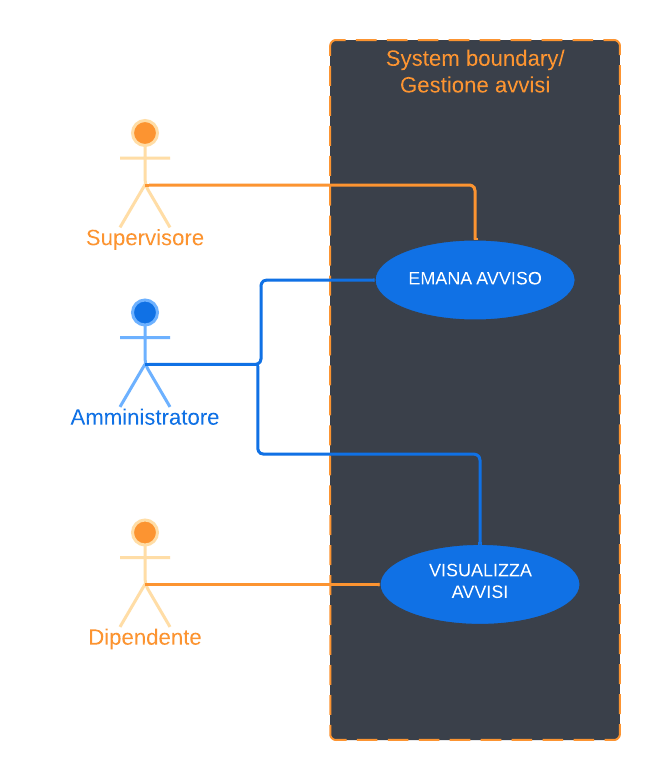
\includegraphics[width=0.8\textwidth]{assets/diagrammi/Use-Case/Gestione avvisi.png}
            \caption{Use Case relativo alla gestione degli avvisi}
            \label{fig:ucdAdvMgmt}
        \end{figure}
\newpage
    \subsubsection{Tabelle di Cockburn} %sezione 2.7
    \begin{flushleft}
        Vengono qui riportate le tabelle di cockburn dei casi d'uso  \emph{\textbf{Aggiungi ristorante}},  
        \emph{\textbf{Aggiungi piatto}},  \emph{\textbf{Prendi ordinazione}},  \emph{\textbf{Visualizza avvisi}}.
    \end{flushleft}

    \begin{center}
      \begin{longtblr}{hlines = {0.9pt}, vlines = {0.9pt}, row{1}={marroneApp!60},colspec = {X[c]X[c]X[c]X[c]}, width = \textwidth,  rowhead=1}

            \textbf{Use Case \#1} & \SetCell[c=3]{c} \textbf{Aggiunta ristorante} \\

            \textbf{Goal in Context} & \SetCell[c=3]{l}{Un admin (proprietario di uno o più ristoranti)\\ vuole aggiungere uno di questi nell'app Ratatuille.}\\

            \textbf{Precodition} & \SetCell[c=3]{l}{Il proprietario deve essere registrato e loggato nell'app come amministratore}\\

            \textbf{Success End Condition} & \SetCell[c=3]{l}{Il proprietario aggiunge correttamente il ristorante}\\

            \textbf{Failed End Condition}  & \SetCell[c=3]{l}{Il proprietario non riesce ad aggiungere il ristorante}\\

            \textbf{Primary Actor}  & \SetCell[c=3]{c}{Amministratore}\\

            \textbf{Trigger}  & \SetCell[c=3]{c}{Preme il pulsante \emph{Aggiungi}}\\

            \SetCell[r=5]{c}\textbf{Description}  & {Step} & {UserAction} & {System}\\
                                                  & {1}    & {L'amministratore preme sul tasto  \emph{"AGGIUNGI RISTORANTE"}\\ sulla schermata \textbf{\emph{M04}}} & \\
                                                  & {2}    &       & {Mostra la schermata \textbf{ \emph{M05}}}\\
                                                  & {3}    &  {Compila i campi necessari per la registrazione del proprio ristorante e preme sul tasto "SALVA" per aggiungere il Ristorante}     & \\
                                                  & {4}    &       & {Ricarica la schermata \textbf{ \emph{M04}} aggiungendo nella lista dei ristoranti l'ultimo appena inserito} \\
            %%% Extensions
            \SetCell[r=2]{c}{\textbf{Extension \#\ 1}\\ L'amministratore non fa nulla e torna indietro}
                                                        & {Step} & {UserAction} & {System}\\
                                                        & {4a}   &  & {Torna alla schermata \textbf{ \emph{M04}}}\\

            \SetCell[r=2]{c}{\textbf{Extension \#2} \\ L'amministratore ha aggiunto un ristorante già presenta nella propria lista di ristoranti} & {Step} & {UserAction} & {System}\\*
                                                        & {4b}   &  & {Mostra uno dei messaggi di errore della schermata \textbf{ \emph{{M0boh}}} restando allo step \textbf{2} dello scenario principale}\\

            \SetCell[r=2]{c}{\textbf{Extension \#3}\\ L'amministratore ha lasciato uno o più campi vuoti}
                                                    & {Step} & {UserAction} & {System}  \\
                                                    & {4c}   &  & {Mostra uno o più dei messaggi di errore della schermata \textbf{ \emph{{M05}}} restando allo step \textbf{2} dello scenario principale}  \\

            \SetCell[r=2]{c}{\textbf{Extension \#4}\\ L'amministratore ha aggiunto un nome troppo corto}
                                                    & {Step} & {UserAction} & {System}\\
                                                    & {4d}   &  & {Mostra il messaggio di errore di fianco al campo  "Nome" della schermata \textbf{ \emph{{M05}}} restando allo step \textbf{2} dello scenario principale} \\

            \SetCell[r=2]{c}{\textbf{Extension \#5}\\ L'amministratore ha aggiunto un numero di coperti non valido}
                                                    & {Step} & {UserAction} & {System}\\
                                                    & {4e}   &  & {Mostra il messaggio di errore di fianco al campo  "Numero di coperti" della schermata \textbf{ \emph{{M05}}} restando allo step \textbf{2} dello scenario principale} \\

            \SetCell[r=2]{c}{\textbf{Extension \#6}\\ L'amministratore ha aggiunto un indirizzo troppo corto}
                                                    & {Step} & {UserAction} & {System}\\*
                                                    & {4f}   &  & {Mostra il messaggio di errore di fianco al campo  "Indirizzo" della schermata \textbf{ \emph{{M05}}} restando allo step \textbf{2} dello scenario principale} \\

            \SetCell[r=2]{c}{\textbf{Extension \#7} \\ L'amministratore ha aggiunto un numero di telefono non valido} & {Step} & {UserAction} & {System}  \\*
                                                    & {4g}   &  & {Mostra il messaggio di errore di fianco al campo "Numero di telefono" della schermata \textbf{ \emph{{M05}}} restando allo step \textbf{2} dello scenario principale} \\

            %%% Subvariations
            \SetCell[r=4]{c}{\textbf{Subvariation \#1} \\ L'amministratore torna indietro completando solo parzialmente i campi} 
                                                        & {Step} & {UserAction} & {System}\\
                                                        & {1} & & {Mostra la schermata \textbf{ \emph{M0boh}}}\\
                                                        & {2} & {Preme su  "SI" } & \\
                                                        & {3} & & {Torna alla schermata \textbf{ \emph{M04}}}\\

            \SetCell[r=4]{c}{\textbf{Subvariation \#2} \\ L'amministratore inizialmente vuole tornare indietro completando solo parzialmente i campi ma cambia idea}
                                                            & {Step} & {UserAction} & {System}\\
                                                            & {1} & & {Mostra la schermata \textbf{ \emph{M0boh}}}\\
                                                            & {2} & {Preme su  "NO" } & \\
                                                            & {3} & & {Torna alla schermata \textbf{ \emph{M05}} allo step \textbf{2} dello scenario principale}\\
      \end{longtblr}
    \end{center}

    \newpage

    \begin{center}
      \begin{longtblr}{hlines = {0.9pt}, vlines = {0.9pt}, row{1}={marroneApp!60},colspec = {X[c]X[c]X[c]X[c]}, width = \textwidth,  rowhead=1}

            \textbf{Use Case \#2} & \SetCell[c=3]{c} \textbf{Prendere un ordine} \\

            \textbf{Goal in Context} & \SetCell[c=3]{l}{Un cameriere vuole prendere l'ordinazione di un tavolo}\\

            \textbf{Precodition} & \SetCell[c=3]{l}{Il cameriere deve essere registrato e loggato nell'app \\ e il ristorante deve avere un menu con dei piatti al suo interno}\\

            \textbf{Success End Condition} & \SetCell[c=3]{l}{Il cameriere prendere correttamente un'ordinazione}\\

            \textbf{Failed End Condition}  & \SetCell[c=3]{l}{Il cameriere non prende l'ordinazione}\\

            \textbf{Primary Actor}  & \SetCell[c=3]{c}{Cameriere}\\

            \textbf{Trigger}  & \SetCell[c=3]{c}{Preme il pulsante \emph{NUOVO ORDINE}}\\

            \SetCell[r=5]{c}\textbf{Description}  & {Step} & {UserAction} & {System}\\
                                                  & {1}    & {Il cameriere preme sul pulsante  \emph{"NUOVO ORDINE"}\\ sulla schermata \textbf{\emph{M11}}} & \\
                                                  & {2}    &       & {Mostra la schermata \textbf{ \emph{M19}} con i vari piatti del menu}\\
                                                  & {3}    &  {Il cameriere seleziona il numero del tavolo, inserisce le portate all'interno dell'ordine e preme il pulsante "\emph{SALVA}"}     & \\
                                                  & {4}    &       & {Torna alla schermata \textbf{ \emph{M11}}} \\
            %%% Extensions
            \SetCell[r=2]{c}{\textbf{Extension \#\ 1}\\ Il cameriere non fa nulla e torna indietro}
                                                        & {Step} & {UserAction} & {System}\\
                                                        & {4a}   &  & {Torna alla schermata \textbf{ \emph{M11}}}\\

            %%% Subvariations
            \SetCell[r=4]{c}{\textbf{Subvariation \#1} \\ Il cameriere torna indietro dopo aver aggiunto \\ dei piatti all'ordine senza salvare} 
                                                        & {Step} & {UserAction} & {System}\\
                                                        & {1} &     & {Mostra la schermata \textbf{ \emph{M0boh}}}\\
                                                        & {2} & {Preme su  "SI" } & \\
                                                        & {3} &     & {Torna alla schermata \textbf{ \emph{M11}}}\\

            \SetCell[r=4]{c}{\textbf{Subvariation \#2} \\ L'amministratore inizialmente vuole tornare indietro completando solo parzialmente i campi ma cambia idea}
                                                            & {Step} & {UserAction} & {System}\\*
                                                            & {1} & & {Mostra la schermata \textbf{ \emph{M0boh}}}\\
                                                            & {2} & {Preme su  "NO" } & \\
                                                            & {3} & & {Torna alla schermata \textbf{ \emph{M11}}}\\
      \end{longtblr}
    \end{center}

    \begin{center}
      \begin{longtblr}{hlines = {0.9pt}, vlines = {0.9pt}, row{1}={marroneApp!60},colspec = {X[c]X[c]X[c]X[c]}, width = \textwidth,  rowhead=1}

            \textbf{Use Case \#3} & \SetCell[c=3]{c} \textbf{Aggiungi piatto al menu} \\

            \textbf{Goal in Context} & \SetCell[c=3]{l}{Un amministratore vuole aggiungere un piatto al proprio menu}\\

            \textbf{Precodition} & \SetCell[c=3]{l}{Il proprietario deve essere registrato e loggato nell'app come amministratore, \\ deve aver aggiunto almeno un ristorante e deve averne creato un menu}\\

            \textbf{Success End Condition} & \SetCell[c=3]{l}{L'amministratore aggiunge correttamente un piatto al suo menu}\\

            \textbf{Failed End Condition}  & \SetCell[c=3]{l}{L'amministratore non riesce ad aggiungere un piatto al suo ristorante}\\

            \textbf{Primary Actor}  & \SetCell[c=3]{c}{Amministratore}\\

            \textbf{Trigger}  & \SetCell[c=3]{c}{Preme il pulsante \emph{Aggiungi prodotto}}\\

            \SetCell[r=5]{c}\textbf{Description}  & {Step} & {UserAction} & {System}\\
                                                  & {1}    & {L'amministratore preme sul pulsante \emph{Aggiungi prodotto}\\ sulla schermata \textbf{ \emph{M08}}} & \\
                                                  & {2}    &       & {Mostra la schermata \textbf{\emph{M18}}}\\
                                                  & {3}    &  {L'amministratore compila il campi del piatto e preme sul pulsante pulsante \emph{OK}}     & \\
                                                  & {4}    &       & {Torna alla schermata \textbf{ \emph{M08}}} \\
            %%% Extensions
            \SetCell[r=2]{c}{\textbf{Extension \#\ 1}\\ L'amministratore non fa nulla e torna indietro}
                                                        & {Step} & {UserAction} & {System}\\
                                                        & {4a}   &  & {Torna alla schermata \textbf{ \emph{M08}}}\\

            \SetCell[r=2]{c}{\textbf{Extension \#\ 2}\\ L'amministratore compila solo parzialmente \\ i campi e preme sul pulsante \emph{OK}}
                                                        & {Step} & {UserAction} & {System}\\
                                                        & {4a}   &  & {Mostra l'errore nella schermata \textbf{\emph{M0boh}}}\\

            %%% Subvariations
            \SetCell[r=6]{c}{\textbf{Subvariation \#1} \\ L'amministratore vuole aggiungere un prodotto \\ preconfezionato al proprio menu} 
                                                        & {Step} & {UserAction} & {System}\\
                                                        & {1} &     & {Mostra la schermata \textbf{ \emph{M18}}}\\
                                                        & {2} & {L'amministratore scrive il nome (completo o parziale)\\di un prodotto e preme il pulsante \emph{Cerca}} & \\
                                                        & {3} &     & {Mostra i prodotti corrispondenti alla ricerca}\\
                                                        & {4} & {L'amministratore seleziona il prodotto desiderato e preme il pulsante \emph{OK}}   & \\
                                                        & {5} &     & {Torna alla schermata \textbf{\emph{M08}}}

      \end{longtblr}
    \end{center}

    \newpage

    \begin{center}
      \begin{longtblr}{hlines = {0.9pt}, vlines = {0.9pt}, row{1}={marroneApp!60},colspec = {X[c]X[c]X[c]X[c]}, width = \textwidth,  rowhead=1}

            \textbf{Use Case \#4} & \SetCell[c=3]{c} \textbf{Visualizza avvisi} \\

            \textbf{Goal in Context} & \SetCell[c=3]{l}{Un dipendente vuole visualizzare un avviso}\\

            \textbf{Precodition} & \SetCell[c=3]{l}{Il dipendente deve essere registrato e loggato nell'app}\\

            \textbf{Success End Condition} & \SetCell[c=3]{l}{Il dipendente visualizza gli avvisi}\\

            \textbf{Failed End Condition}  & \SetCell[c=3]{l}{Il dipendente non riesce a visualizzare i propri avvisi}\\

            \textbf{Primary Actor}  & \SetCell[c=3]{c}{Dipendente}\\

            \textbf{Trigger}  & \SetCell[c=3]{c}{Preme il pulsante \emph{Avvisi} nella propria Dashboard}\\

            \SetCell[r=3]{c}\textbf{Description}  
                                                  & {Step} & {UserAction} & {System}\\
                                                  & {1}    & {Il Dipendente preme sul pulsante \emph{Avvisi} sulla schermata \textbf{\emph{M11}} o \textbf{\emph{M09}} o \textbf{\emph{M12}}} & \\
                                                  & {2}    &       & {Mostra la schermata \textbf{\emph{M21}}}  \\

            %%% Extensions
            \SetCell[r=2]{c}{\textbf{Extension \#\ 1}\\ Non ci sono avvisi da mostrare}
                                                        & {Step} & {UserAction} & {System}\\
                                                        & {4a}   &  & {Mostra la schermata \textbf{\emph{M21}}}\\

            %%% Subvariations
            \SetCell[r=3]{c}{\textbf{Subvariation \#1} \\ Il Dipendente vuole marcare un avviso come visualizzato} 
                                                        & {Step} & {UserAction} & {System}\\
                                                        & {1} & {Il Dipendente scorre col dito sull'avviso}   & \\
                                                        & {2} &       & {Aggiorna la schermata \textbf{\emph{M21}} eliminando l'avviso} \\

      \end{longtblr}
    \end{center}

    \newpage
    \subsection{Mock-up dell'applicazione}
    \begin{flushleft}
        Qui vengono presentati i mockup relativi all'applicazione.
    \end{flushleft}
    \subsubsection{Homepage dell'applicazione}
        \begin{figure}[H]
          \centering
          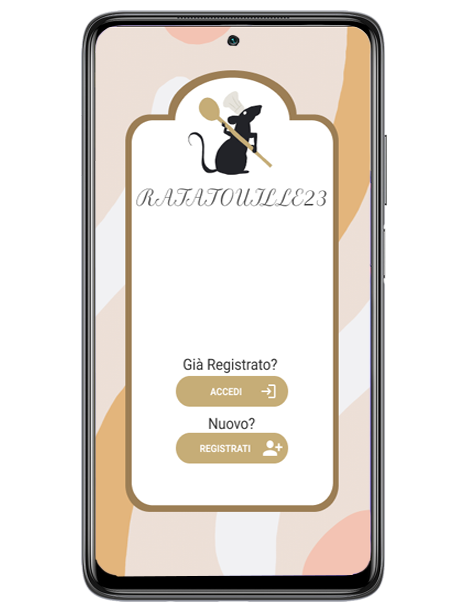
\includegraphics[scale=0.5]{assets/Mockup/Mockup_Homepage.png}
          \caption{\textbf{M01}: Homepage dell'applicazione}\label{fig:Mockup_Homepage}
        \end{figure}
        \begin{flushleft}
            \textbf{ID} \ \Large{\textit{\textbf{M01}}}\\
        \end{flushleft}

        \textbf{Componenti}:

        \begin{center}
          \begin{tblr}{hlines = {0.9pt}, vlines = {0.9pt}, row{1} = {marroneApp!60}, colspec = {X[c]X[c]X[c]}, width = \textwidth}
            \textbf{Tipo}  &   \textbf{Nome} & \textbf{Funzione} \\
            Bottone        &   ACCEDI        & Quando cliccato porta alla schermata \textit{\textbf{M02}} \\
            Bottone        &   REGISTRATI   & Quando cliccato porta alla schermata \textit{\textbf{M03}}  \\
          \end{tblr}
        \end{center}
        
        \newpage

        \subsubsection{Schermata di accesso nel sistema}
            \begin{figure}[H]
                \centering
                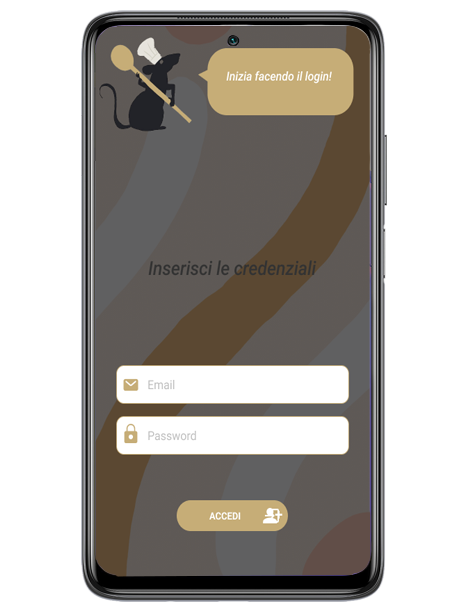
\includegraphics[scale=0.5]{assets/Mockup/Mockup_Accesso.png}
                \caption{\textbf{M02}: Schermata di accesso nel sistema}\label{fig:Mockup_Login}
            \end{figure}
            \begin{flushleft}
                \textbf{ID} \ \Large{\textit{\textbf{M02}}}\\
            \end{flushleft}

            \textbf{Componenti}:

            \begin{center}
              \begin{tblr}{hlines = {0.9pt}, vlines = {0.9pt}, row{1} = {marroneApp!60}, colspec = {X[c]X[c]X[c]}, width = \textwidth}
                \textbf{Tipo}   &   \textbf{Nome}   &   \textbf{Funzione} \\
                Edit Text       &   EMAIL &   Permette l'inserimento dell'email dell'utente \\
                Edit Text       &   PASSWORD  &  Permette l'inserimento della password dell'utente  \\
                Bottone         &   ENTRA   & Quando cliccato porta alla schermata \textit{\textbf{M04}} se admin, \textit{\textbf{M09}} se supervisore, \textit{\textbf{M11}} se cameriere,   \\
              \end{tblr}
            \end{center}

        \newpage
        \subsubsection{Schermata di registrazione nel sistema}
        \begin{figure}[H]
          \centering
          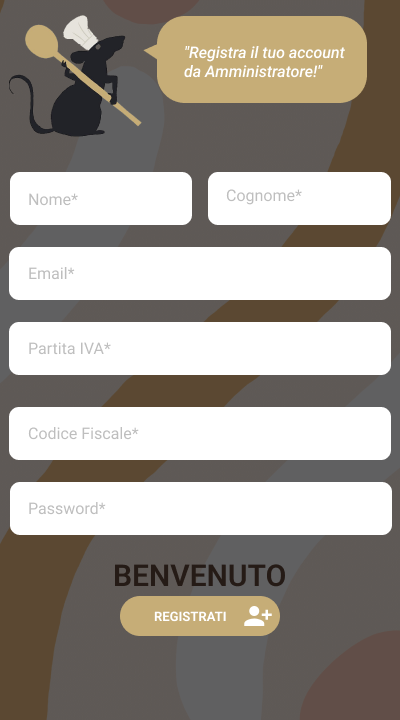
\includegraphics[scale=0.25]{assets/Mockup/Mockup_Register.png}
          \caption{\textbf{M03}: Schermata di registrazione nel sistema}\label{fig:Mockup_Register}
        \end{figure}

        \begin{flushleft}
          \textbf{ID} \ \Large{\textit{\textbf{M03}}}\\
          \large{\textit{Nota}: la schermata di registrazione è valida solo per gli admin proprietari dei ristoranti, in quanto sono poi loro a registrare i dipendenti.}\\
        \end{flushleft}

        \textbf{Componenti}:

            \begin{center}
              \begin{longtblr}{hlines = {0.9pt}, vlines = {0.9pt}, row{1} = {marroneApp!60}, colspec = {X[c]X[c]X[c]}, width = \textwidth, rowhead=1}
                \textbf{Tipo}   &   \textbf{Nome}   &   \textbf{Funzione} \\
                Edit Text    &   NOME    &   Permette di inserire il nome dell'admin \\
                Edit Text & COGNOME   &  Permette di inserire il cognome dell'admin \\
                Edit Text    &   PASSWORD    &   Permette di inserire una password per l'admin \\
                Edit Text    &   EMAIL   &   Permette di inserire l'email dell'admin \\
                Edit Text    & CODICE FISCALE    & Permette di inserire il codice fiscale dell'admin \\
                Edit Text    &   P.IVA   & Permette di inserire la partita IVA dell'admin \\
                Bottone &   REGISTRATI  & Quando cliccato riporta alla schermata \textit{\textbf{M01}} per permettere l'accesso \\
              \end{longtblr}
            \end{center}
        \newpage
        \subsubsection{Schermata home per gli admin}
        \begin{figure}[H]
            \centering
            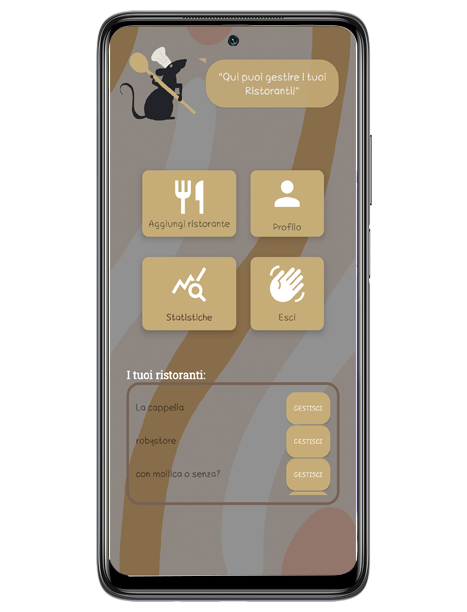
\includegraphics[scale=0.35]{assets/Mockup/Mockup_AdminDash.png}
            \caption{\textbf{M04}: Schermata home per gli admin}\label{fig:Mockup_AdminDashboard}
        \end{figure}
        \begin{flushleft}
            \textbf{ID} \ \Large{\textit{\textbf{M04}}} \\
        \end{flushleft}
        \textbf{Componenti}:

            \begin{center}
                \begin{longtblr}{hlines = {0.9pt}, vlines = {0.9pt}, row{1} = {marroneApp!60}, colspec = {X[c]X[c]X[c]}, width = \textwidth, rowhead=1}
                \textbf{Tipo}   &   \textbf{Nome}   &   \textbf{Funzione} \\
                ScrollView &   I TUOI RISTORANTI    &   Visualizza ed eventualmente permette la modifica dei ristoranti registrati\\
                Bottone    &   AGGIUNGI RISTORANTE  &   Quando cliccato porta alla schermata \textit{\textbf{M05}} \\
                Bottone    &   MODIFICA   &   Quando cliccato porta alla schermata \textit{\textbf{M06}} \\
                Bottone    &   PROFILO    &   Quando cliccato porta alla schermata \textit{\textbf{M13}} \\
                Bottone    &   ESCI       &   Quando cliccato mostra la schermata \textit{\textbf{M10}} \\
                Bottone    &   STATISTICHE &  Quando cliccato porta alla schermata \textit{\textbf{M0bho}} \\
                \end{longtblr}
            \end{center}
        \newpage

        \subsubsection{Schermata di registrazione di un nuovo ristorante}
        \begin{figure}[H]
            \centering
            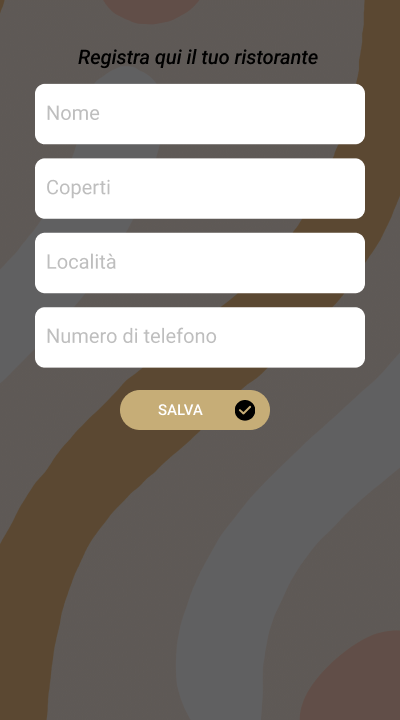
\includegraphics[scale=0.35]{assets/Mockup/Mockup_SaveResturant.png}
            \caption{\textbf{M05}: Schermata di registrazione di un nuovo ristorante}\label{fig:Mockup_AddResturant}
        \end{figure}
        \begin{flushleft}
            \textbf{ID} \ \Large{\textit{\textbf{M05}}}
        \end{flushleft}
        \textbf{Componenti}:

        \begin{center}
          \begin{tblr}{hlines = {0.9pt}, vlines = {0.9pt}, row{1} = {marroneApp!60}, colspec = {X[c]X[c]X[c]}, width = \textwidth}
            \textbf{Tipo}  &   \textbf{Nome}  & \textbf{Funzione} \\
            Edit Text      &   NOME           & Permette di inserire il nome del nuovo ristorante\\
            Edit Text      &   LOCALITA'      & Permette di inserire la località del nuovo ristorante\\
            Edit Text      &   COPERTI        & Permette di inserire il n° dei coperti del nuovo ristorante\\
            Edit Text      &   NUMERO DI TELEFONO & Permette di inserire il contatto telefonico del ristorante \\
            Bottone        &   SALVA          & Quando cliccato salva il nuovo ristorante nel database e torna alla schermata \textit{\textbf{M04}} \\
          \end{tblr}
        \end{center}
        \newpage
        \subsubsection{Schermata di modifica di un ristorante}
        \begin{figure}[H]
            \centering
            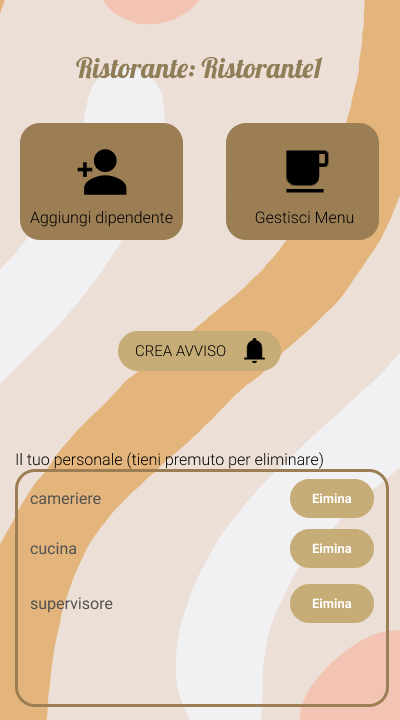
\includegraphics[scale=0.5]{assets/Mockup/Mockup_ResturantDash.png}
            \caption{\textbf{M06}: Schermata di modifica di un ristorante}\label{fig:Mockup_ResturantManager}
        \end{figure}
        \begin{flushleft}
            \textbf{ID} \ \Large{\textit{\textbf{M06}}}
        \end{flushleft}

        \textbf{Componenti}:

          \begin{center}
            \begin{tblr}{hlines = {0.9pt}, vlines = {0.9pt}, row{1} = {marroneApp!60}, colspec = {X[c]X[c]X[c]}, width = \textwidth}
              \textbf{Tipo}  &   \textbf{Nome}  & \textbf{Funzione} \\
              \textbf{Tipo}   &   \textbf{Nome}   &   \textbf{Funzione} \\
              Bottone   &   AGGIUNGI DIPENDENTE &   Quando cliccato porta alla schermata \textit{\textbf{M07}}\\
              Bottone   &   GESTISCI MENU &   Quando cliccato porta alla schermata \textit{\textbf{M08}}\\
              ScrollView  & IL TUO PERSONALE  & Mostra il personale che lavora nel ristorante \\
              Bottone   &   CREA AVVISO   &   Quando cliccato mostra la schermata \textit{\textbf{M17}} \\  
            \end{tblr}
          \end{center}

        \newpage

        \subsubsection{Schermata di registrazione di un nuovo dipendente}
        \begin{figure}[H]
            \centering
            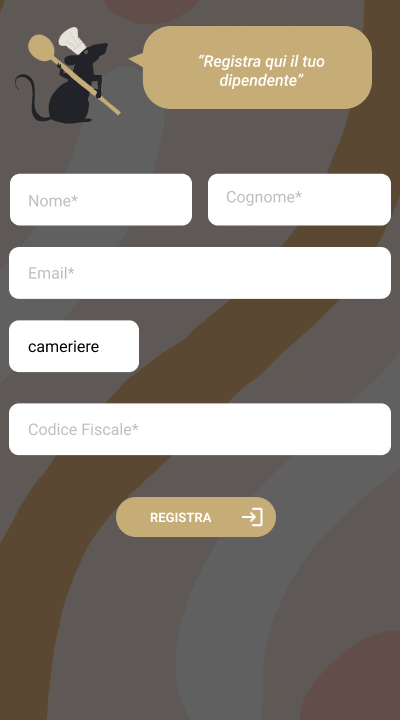
\includegraphics[scale=0.35]{assets/Mockup/Mockup_SaveWorker.png}
            \caption{\textbf{M07}: Schermata di registrazione di un nuovo dipendente}\label{fig:Mockup_SaveWaiter}
        \end{figure}
        \begin{flushleft}
            \textbf{ID} \ \Large{\textit{\textbf{M07}}}
        \end{flushleft}
        \textbf{Componenti}:

        \begin{center}
          \begin{tblr}{hlines = {0.9pt}, vlines = {0.9pt}, row{1} = {marroneApp!60}, colspec = {X[c]X[c]X[c]}, width = \textwidth}
            \textbf{Tipo}   &   \textbf{Nome}   &   \textbf{Funzione} \\
            Edit Text   &   NOME    &   Permette di inserire il nome del nuovo dipendente\\
            Edit Text   &   COGNOME   &   Permette di inserire il cognome del nuovo dipendente\\
            Edit Text   &   EMAIL   & Permette di inserire l'email del nuovo dipendente\\
            Edit Text   &   CODICE FISCALE    &   Permette di inserire il codice fiscale del nuovo dipendente \\
            Spinner &   {cameriere\\ (default)}    &   Permette di inserire il ruolo del nuovo dipendente \\
            Bottone &   REGISTRA    &   Quando cliccato, se tutti i dati sono corretti, riporta alla schermata \textit{\textbf{M04}} registrando il nuovo dipendente \\
          \end{tblr}
        \end{center}

        \newpage

        \subsubsection{Schermata di gestione del menù}
        \begin{figure}[H]
            \centering
            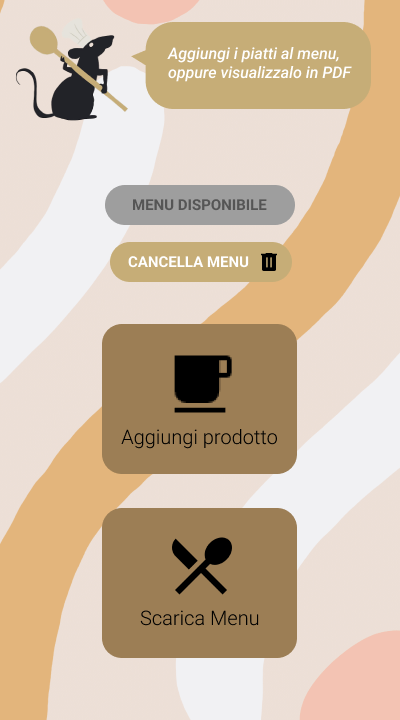
\includegraphics[scale=0.5]{assets/Mockup/Mockup_MenuManager.png}
            \caption{\textbf{M08}: Schermata di gestione del menù}\label{fig:Mockup_MenuManager}
        \end{figure}
        \begin{flushleft}
            \textbf{ID} \ \Large{\textit{\textbf{M08}}}
        \end{flushleft}
        \textbf{Componenti}:

        \begin{center}
          \begin{tblr}{hlines = {0.9pt}, vlines = {0.9pt}, row{1} = {marroneApp!60}, colspec = {X[c]X[c]X[c]}, width = \textwidth}
            \textbf{Tipo}   &   \textbf{Nome}   &   \textbf{Funzione} \\
            Bottone   &   AGGIUNGI PRODOTTO    &   Quando cliccato porta alla schermata \textit{\textbf{M18}}\\
            Edit Text   &   SCARICA MENU   &   Permette di generare il menù e salvarlo sul dispositivo in formato PDF\\
            Bottone   &   CREA MENU       &   Quando cliccato permette di creare un menu (se non è gia stato creato)
          \end{tblr}
        \end{center}

        \newpage

        \subsubsection{Schermata home per i supervisori}
          \begin{figure}[H]
              \centering
              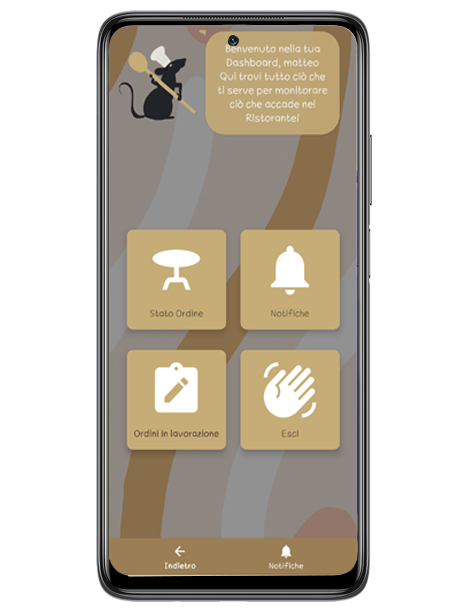
\includegraphics[scale=2.5]{assets/Mockup/Mockup_HypervisorDash.png}
              \caption*{\textbf{M09}: Schermata home dei supervisori}\label{fig:Mockup_HypervisorDash}
          \end{figure}

          \begin{flushleft}
              \textbf{ID}   \ \Large{\textit{\textbf{M09}}}
          \end{flushleft}

          \textbf{Componenti}:

          \begin{center}
              \begin{tblr}{hlines = {0.9pt}, vlines = {0.9pt}, row{1} = {marroneApp!60}, colspec = {X[c]X[c]X[c]}, width = \textwidth}
                \textbf{Tipo}   &   \textbf{Nome}   &   \textbf{Funzione} \\
                Bottone   &   STATO ORDINE    &   Quando cliccato porta alla schermata \textit{\textbf{M0bho}} \\
                Bottone   &   NOTIFICHE       &   Quando cliccato \\ %Inserire cosa fa
                Bottone   &   ORDINI IN LAVORAZIONE & \\ %Questo non l'ho capito
                Bottone   &   ESCI    &   Quando cliccato porta alla schermata \textit{\textbf{M10}} \\
                %TODO: Vedere la barra sotto come rappresentarla
              \end{tblr}
          \end{center}

        \newpage

        \subsubsection{Schermata di conferma di logout}
          \begin{figure}[H]
            \centering
            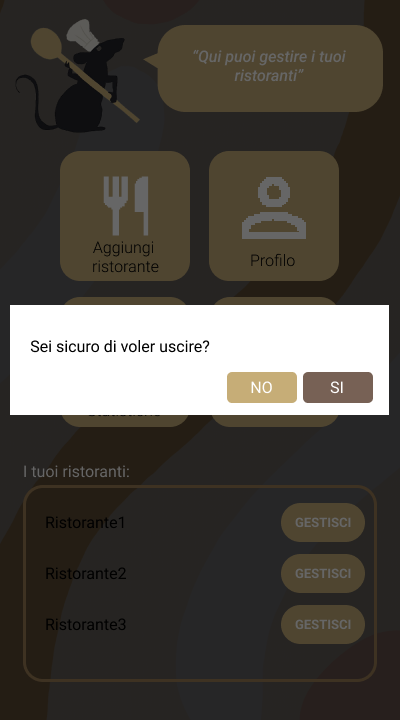
\includegraphics[scale=2]{assets/Mockup/Mockup_ExitDialog.png}
            \caption*{\textbf{M10}: Schermata di conferma logout}\label{fig:Mockup_ExitDialog}
          \end{figure}

          \begin{flushleft}
            \textbf{ID}   \ \Large{\textit{\textbf{M10}}}
          \end{flushleft}

          \textbf{Componenti}:

          \begin{center}
            \begin{tblr}{hlines = {0.9pt}, vlines = {0.9pt}, row{1} = {marroneApp!60}, colspec = {X[c]X[c]X[c]}, width = \textwidth}
              \textbf{Tipo}   &   \textbf{Nome}   &   \textbf{Funzione} \\
              Bottone         &   SI      &   Quando cliccato porta alla schermata \textit{\textbf{M02}} \\
              Bottone         &   NO      &   Quando cliccato resta nella schermata corrente \\
            \end{tblr}
          \end{center}
        
        \newpage

        \subsubsection{Schermata home per i camerieri}
          \begin{figure}[H]
            \centering
            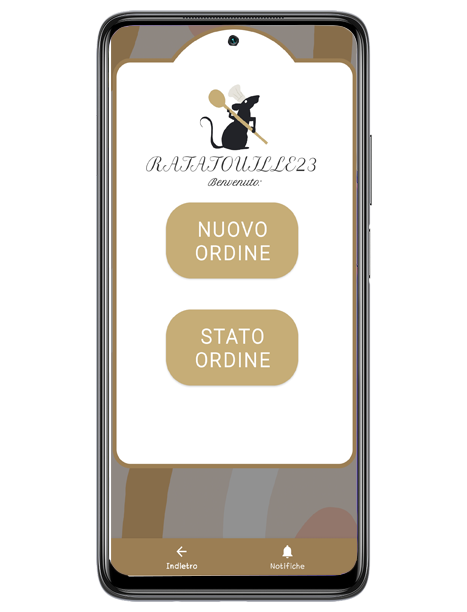
\includegraphics[scale=2]{assets/Mockup/Mockup_WaiterDash.png}
            \caption*{\textbf{M11}: Schermata home per i camerieri}\label{fig:Mockup_WaiterDash}
          \end{figure}

          \begin{flushleft}
            \textbf{ID}   \ \Large{\textit{\textbf{M11}}}
          \end{flushleft}

          \textbf{Componenti}:
          
          \begin{center}
            \begin{tblr}{hlines = {0.9pt}, vlines = {0.9pt}, row{1} = {marroneApp!60}, colspec = {X[c]X[c]X[c]}, width = \textwidth}
              \textbf{Tipo}   &   \textbf{Nome}   &   \textbf{Funzione} \\
              Bottone     &   NUOVO ORDINE    &   Quando cliccato porta alla schermata \textit{\textbf{M19}} \\
              Bottone     &   STATO ORDINE    &   Quando cliccato porta alla schermata \textit{\textbf{M0bho}} \\
              % TODO: Vedere la barra sotto come rappresentarla
            \end{tblr}
          \end{center}

        \newpage

        \subsubsection{Schermata home per la cucina}
  
            \begin{flushleft}
              \textbf{ID}   \ \Large{\textit{\textbf{M12}}}
            \end{flushleft}
  
            \textbf{Componenti}:
            
            \begin{center}
              \begin{tblr}{hlines = {0.9pt}, vlines = {0.9pt}, row{1} = {marroneApp!60}, colspec = {X[c]X[c]X[c]}, width = \textwidth}
                \textbf{Tipo}   &   \textbf{Nome}   &   \textbf{Funzione} \\
  
              \end{tblr}
            \end{center}

            \newpage

            \subsubsection{Schermata di visualizzazione del profilo}
              \begin{figure}[H]
                \centering
                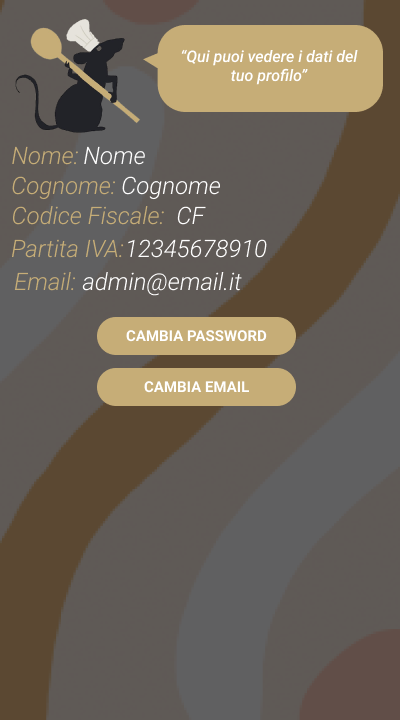
\includegraphics[scale=2.5]{assets/Mockup/Mockup_Profile.png}
                \caption*{\textbf{M13}: Schermata visualizzazione profilo}\label{fig:Mockup_Profile}
              \end{figure}
    
              \begin{flushleft}
                \textbf{ID}   \ \Large{\textit{\textbf{M13}}}
              \end{flushleft}
    
              \textbf{Componenti}:
              
              \begin{center}
                \begin{tblr}{hlines = {0.9pt}, vlines = {0.9pt}, row{1} = {marroneApp!60}, colspec = {X[c]X[c]X[c]}, width = \textwidth}
                  \textbf{Tipo}   &   \textbf{Nome}   &   \textbf{Funzione} \\
                  Bottone     &   CAMBIA PASSWORD   &   Quando cliccato mostra la schermata \textit{\textbf{M14}}  \\
                  Bottone     &   CAMBIA EMAIL   &   Quando cliccato mostra la schermata \textit{\textbf{M15}}  \\    
                \end{tblr}
              \end{center}

              \newpage

              \subsubsection{Schermata di cambio password per gli admin}
                \begin{figure}[H]
                  \centering
                  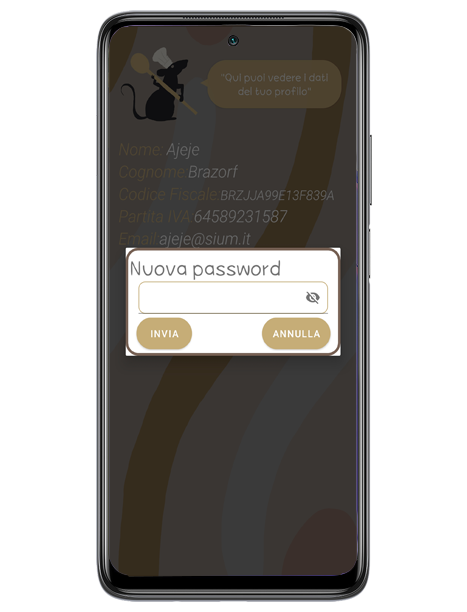
\includegraphics[scale=2.5]{assets/Mockup/Mockup_AdminChangePass.png}
                  \caption*{\textbf{M14}: Schermata cambio password admin}\label{fig:Mockup_AdminChangePass}
                \end{figure}
      
                \begin{flushleft}
                  \textbf{ID}   \ \Large{\textit{\textbf{M14}}}
                \end{flushleft}
      
                \textbf{Componenti}:
                
                \begin{center}
                  \begin{tblr}{hlines = {0.9pt}, vlines = {0.9pt}, row{1} = {marroneApp!60}, colspec = {X[c]X[c]X[c]}, width = \textwidth}
                    \textbf{Tipo}   &   \textbf{Nome}   &   \textbf{Funzione} \\
                    Edit Text     &   NUOVA PASSWORD    &   Permette di inserire la nuova password per l'account dell'admin   \\
                    Bottone     &   ANNULLA   &   Quando cliccato torna alla schermata \textit{\textbf{M13}} senza effettuare modifiche  \\
                    Bottone     &   INVIA   &   Quando cliccato torna alla schermata \textit{\textbf{M13}} modificando la password dell'account  \\
                  \end{tblr}
                \end{center}

                \newpage

                \subsubsection{Schermata di cambio email per gli admin}
                  \begin{figure}[H]
                    \centering
                    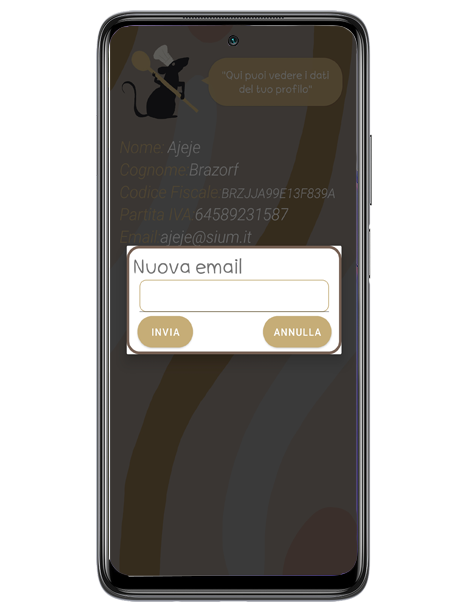
\includegraphics[scale=2.5]{assets/Mockup/Mockup_AdminChangeMail.png}
                    \caption*{\textbf{M15}: Schermata cambio email admin}\label{fig:Mockup_AdminChangeMail}
                  \end{figure}
        
                  \begin{flushleft}
                    \textbf{ID}   \ \Large{\textit{\textbf{M15}}}
                  \end{flushleft}
        
                  \textbf{Componenti}:
                  
                  \begin{center}
                    \begin{tblr}{hlines = {0.9pt}, vlines = {0.9pt}, row{1} = {marroneApp!60}, colspec = {X[c]X[c]X[c]}, width = \textwidth}
                      \textbf{Tipo}   &   \textbf{Nome}   &   \textbf{Funzione} \\
                      Edit Text   &   NUOVA EMAIL   &   Permette di inserire la nuova email per l'account dell'admin  \\
                      Bottone     &   ANNULLA   &   Quando cliccato torna alla schermata \textit{\textbf{M13}} senza effettuare modifiche  \\
                      Bottone     &   INVIA   &   Quando cliccato torna alla schermata \textit{\textbf{M13}} modificando l'email dell'account  \\
                    \end{tblr}
                  \end{center}

                \newpage

                \subsubsection{Schermata di cambio password per i dipendenti al primo accesso}
                    \begin{figure}[H]
                      \centering
                      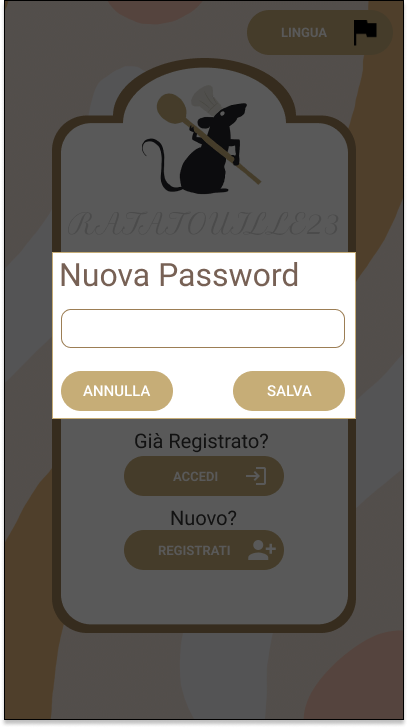
\includegraphics[scale=2]{assets/Mockup/Mockup_WorkerChangePass.png}
                      \caption*{\textbf{M16}: Schermata cambio password dipendenti}\label{fig:Mockup_WorkerChangePass}
                    \end{figure}
          
                    \begin{flushleft}
                      \textbf{ID}   \ \Large{\textit{\textbf{M16}}}
                    \end{flushleft}
          
                    \textbf{Componenti}:
                    
                    \begin{center}
                      \begin{tblr}{hlines = {0.9pt}, vlines = {0.9pt}, row{1} = {marroneApp!60}, colspec = {X[c]X[c]X[c]}, width = \textwidth}
                        \textbf{Tipo}   &   \textbf{Nome}   &   \textbf{Funzione} \\
                        Edit Text   &   NUOVA PASSWORD   &   Permette di inserire la nuova password per l'account del dipendente  \\
                        Bottone     &   ANNULLA   &   Quando cliccato torna alla schermata \textit{\textbf{M02}} senza effettuare modifiche  \\
                        Bottone     &   INVIA   &   Quando cliccato porta alla schermata \textit{\textbf{M09}} se è supervisore, \textit{\textbf{M11}} se è cameriere, \textit{\textbf{M12}} se è un account di cucina, modificando l'email dell'account  \\
                      \end{tblr}
                    \end{center}

                  \newpage

                  \subsubsection{Schermata di creazione degli avvisi}
                      \begin{figure}[H]
                        \centering
                        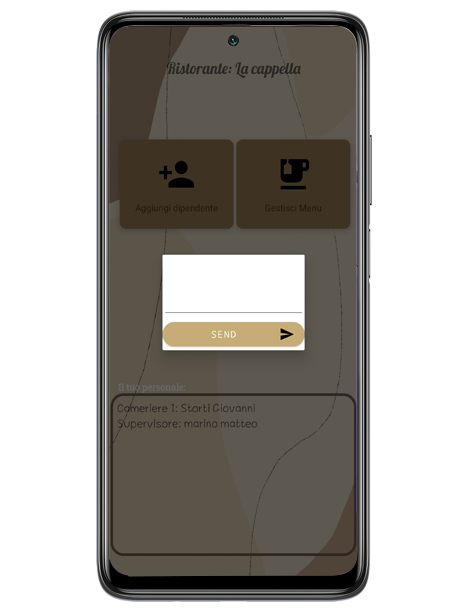
\includegraphics[scale=2.5]{assets/Mockup/Mockup_SaveAdv.png}
                        \caption*{\textbf{M17}: Schermata creazione avvisi}\label{fig:Mockup_SaveAdv}
                      \end{figure}
            
                      \begin{flushleft}
                        \textbf{ID}   \ \Large{\textit{\textbf{M17}}}
                      \end{flushleft}
            
                      \textbf{Componenti}:

                      \begin{center}
                        \begin{tblr}{hlines = {0.9pt}, vlines = {0.9pt}, row{1} = {marroneApp!60}, colspec = {X[c]X[c]X[c]}, width = \textwidth}
                          \textbf{Tipo}   &   \textbf{Nome}   &   \textbf{Funzione} \\
                          Edit Text     &   AVVISO    &   Permette di inserire il testo dell'avviso \\
                          Bottone       &   SEND      &   Quando cliccato torna alla schermata \textit{\textbf{M06}} inviando l'avviso \\
                        \end{tblr}
                      \end{center}

                    \newpage

                    \subsubsection{Schermata di aggiunta piatti al menù}
                        \begin{figure}[H]
                          \centering
                          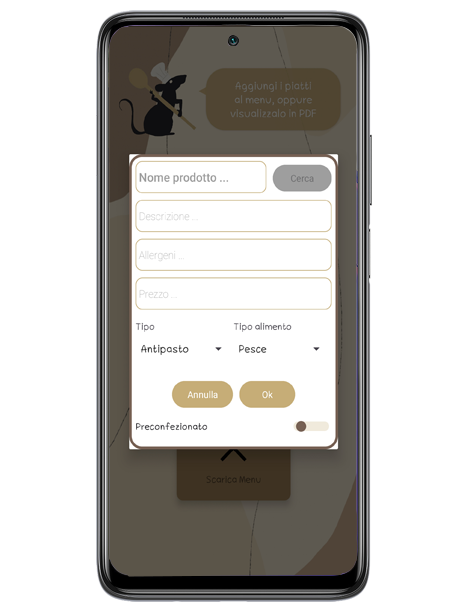
\includegraphics[scale=2]{assets/Mockup/Mockup_AddPlate.png}
                          \caption*{\textbf{M18}: Schermata aggiunta piatti al menù}\label{fig:Mockup_AddPlate}
                        \end{figure}
              
                        \begin{flushleft}
                          \textbf{ID}   \ \Large{\textit{\textbf{M18}}}
                        \end{flushleft}
              
                        \textbf{Componenti}:
                        
                        \begin{center}
                          \begin{longtblr}{hlines = {0.9pt}, vlines = {0.9pt}, row{1} = {marroneApp!60}, colspec = {X[c]X[c]X[c]}, width = \textwidth, rowhead=1}
                            \textbf{Tipo}   &   \textbf{Nome}   &   \textbf{Funzione} \\
                            EditText        &   NOME PRODOTTO   &   Permette di inserire il titolo del prodotto da inserire \\
                            EditText        &   DESCRIZIONE     &   Permette di inserire la descrizione del prodotto da Inserire  \\
                            EditText        &   ALLERGENI       &   Permette di inserire gli allergeni contenuti nel prodotto \\
                            EditText        &   PREZZO          &   Permette di inserire il prezzo del prodotto \\
                            Spinner         &   TIPO            &   Permette di inserire il tipo di portata (antipasto, primo, ...) \\
                            Spinner         &   TIPO DI ALIMENTO &  Permette di inserire il tipo di alimento (carne, pesce, ...)  \\
                            Bottone         &   CERCA           &   Quando cliccato, ricerca il prodotto scritto nel database di OpenFoodFacts  \\
                            Bottone         &   OK              &   Quando cliccato, ritorna alla schermata \textit{\textbf{M08}} salvando nel menu il prodotto \\
                            Bottone         &   ANNULLA         &   Quando cliccate, ritorna alla schermata \textit{\textbf{M08}} senza salvare il prodotto \\  
                            Selettore       &   PRECONFEZIONATO &   Se selezionato, indica che l'oggetto è di tipo preconfezionato(bibita, ...) \\
                          \end{longtblr}
                        \end{center}

                      \newpage

                    \subsubsection{Schermata di aggiunta ordini}
                          \begin{figure}[H]
                            \centering
                            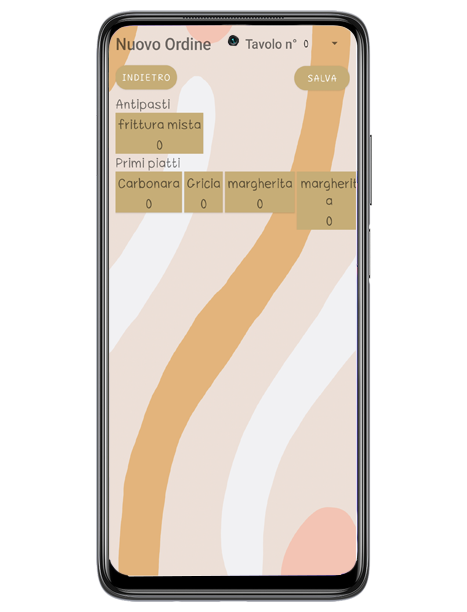
\includegraphics[scale=2]{assets/Mockup/Mockup_AddOrder.png}
                            \caption*{\textbf{M19}: Schermata aggiunta ordini}\label{fig:Mockup_WaiterDash}
                          \end{figure}
                
                          \begin{flushleft}
                            \textbf{ID}   \ \Large{\textit{\textbf{M19}}}
                          \end{flushleft}
                
                          \textbf{Componenti}:
                          
                          \begin{center}
                            \begin{tblr}{hlines = {0.9pt}, vlines = {0.9pt}, row{1} = {marroneApp!60}, colspec = {X[c]X[c]X[c]}, width = \textwidth}
                              \textbf{Tipo}   &   \textbf{Nome}   &   \textbf{Funzione} \\
                              ScrollView      &   PIATTI    &   Visualizza la lista dei piatti del menù del ristorante, dove ogni piatto si può cliccare per aggiungerlo all'ordine \\
                              Bottone         &   SALVA     &   Quando cliccato porta alla schermata \textit{\textbf{M11}} inviando l'ordine \\
                              Bottone         &   INDIETRO  &   Quando cliccato porta alla schermata \textit{\textbf{M11}} senza effettuare nessuna azione \\
                            \end{tblr}
                          \end{center}
    \subsection{Valutazione dell'usabilità}

    \begin{flushleft}
       Per la valutazione dell'usabilità del nostro applicativo a priori, cioè prima della fase di sviluppo vera a propria,
       abbiamo deciso di imporci come linee guida le euristiche di Nielsen.
       Ne sono 10, ma vorremmo richiamare l'attenzione su alcune di esse nello specifico:
        \begin{itemize}
            \item \textit{Visibilità dello stato del sistema.} Il sistema presentava una discreta mancanza di feedback, che prevediamo di colmare con elementi quali Dialog, Toast, AlertDialog e SnackBar.
            \item \textit{Prevenzione degli errori.} Il sistema reagisce in maniera controllata e predeterminata alle situazioni di errori che gli utenti possono causare. Nulla è lasciato al caso, ed è, nelle build provate dal team, gestita qualsiasi azione eseguibile dagli utenti.
            \item \textit{Riconoscere piuttosto che ricordare.} La nostra app è dotata di sezioni ben distinte, interfacce dinamiche a seconda del tipo di utente che le usa, e icone e testi ecplicativi dell'azione che si va a intrapendere.
            \item \textit{Guida e documentazione.} E' presente un simpatico topolino (che richiama il logo dell'app) che consiglia tramite vignette e piccoli dialoghi le azioni che si possono intraprendere. Inoltre ci sono piccole note come campi obbligatori ecc.
        \end{itemize}
    \end{flushleft}

    \begin{figure}[H]
        \centering
        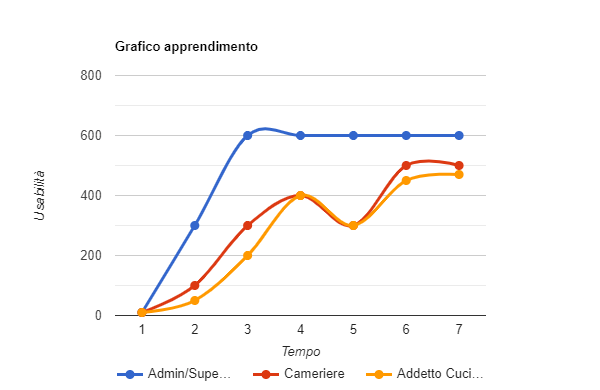
\includegraphics[scale=0.6]{assets/immagini varie/grafico usabilita.png}
        \caption{\textbf{Grafico}: Usabilità}\label{fig:Usabilità_graph}
    \end{figure}
    \subsection{Individuazione target d'utenti}
    \begin{flushleft}
        La conoscenza dell'utente finale è di importanza fondamentale per chi progetta sistemi software di questo tipo. La grande diversità degli esseri umani
        fa sì che, anche considerando compiti e contesti d'uso simili, un oggetto potrebbe risultare usabile per un certo utente e
        del tutto inusabile per un altro.\\
        Sicuramente, in base alle richieste del committente abbiamo subito individuato 4 principali categorie di utenti utilizzatori dell'app:
        \vspace{0.5cm}
       
        \textbf{Admin:} Amministratore e proprietario del ristorante. Una persona che deve avere tutto sotto controllo, può gestire le sue attività nonchè i 
        dipendenti che ne fanno parte, aggiungerne di nuovi e talvolta, purtroppo, eliminarli.
        \vspace{1cm}

        \textbf{Supervisore:} Dopo l'amministratore, è, nella "gerarchia" da noi definita, la seconda persona con più funzioni disponibili in-app. 
        Anch'esso dispone di una dashboard completa sullo stile dell'admin.
        \vspace{1cm}

        \textbf{Cameriere/Addetto sala:} Senza la figura del cameriere un'attività di ristorazione non va avanti. Sappiamo quant'è importante fornire a questi ultimi
        un applicativo funzionale, facile da usare e da apprendere: per questo la sua interfaccia è ottimizzata per un palmare o smartphone compatto.
        \vspace{1cm}


        \textbf{Addetto Cucina:} Riceve tutti gli ordini dai camerieri e li inoltra alla cucina. Anche lui dispone di un'interfaccia semplice e dinamica che perfettamente si adatta al suo ruolo nell'attività.
        \vspace{0.5cm}        
        
        Tutto ciò è reso possibile da uno sviluppo che va incontro alle esigenze dei diversi utenti. La nostra interfaccia riconosce il tipo di utente che logga e cambia
        in base alle sue esigenze. 

    \end{flushleft}


    \begin{figure}[H]
        \centering
        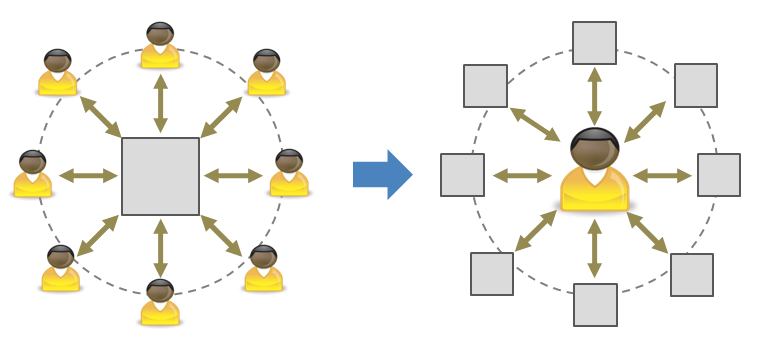
\includegraphics[scale=0.5]{assets/immagini varie/target utenti.png}
        \caption*{\textbf{Figura}: Da una visione centrata sul sistema a una visione centrata sull’utente}\label{fig:target_utenti}
    \end{figure}
    \subsection{Glossario}
    \begin{flushleft}
        In questa sezione vengono chiariti alcuni termini usati all'interno della documentazione, per rendere la lettura accessibile
        anche ai non esperti del settore.
    \end{flushleft}

    \begin{itemize}
        \item \emph{RecyclerView:} potente approccio nella risoluzione di un problema comune: la creazione di liste per la visualizzazione (su Android) di dati ottenuti da un servizio remoto o da un database locale.
        \item \emph{Adapter:} Un oggetto di tipo adapter in Android rappresenta un ponte tra un' AdapterView e i dati che questa deve rappresentare.
        \item \emph{Dialog:} Tipo di popup che il sistema Android mette a disposizione che mostra una finestra di dialog personalizzabile.
        \item \emph{Spring Boot:} Spring è uno strumento che permette a noi programmatori di usare il linguaggio di programmazione ad oggetti java per scrivere ottime app lato server.
        \item \emph{JPA:} Le Java Persistence API, talvolta riferite come JPA, sono un framework per il linguaggio di programmazione Java che si occupa della gestione della persistenza dei dati di un DBMS relazionale
        \item \emph{MVC:} Pattern Model-View-Controller.
        \item \emph{Three-Tier Architecture:} l'espressione architettura three-tier ("a tre strati") indica una particolare architettura software e hardware di tipo multi-tier per l'esecuzione di un'applicazione web che prevede la suddivisione dell'applicazione in tre diversi 
        moduli o strati dedicati rispettivamente alla interfaccia utente, alla logica funzionale (business logic) e alla gestione dei dati persistenti. Android e Spring-Boot ne supportano i principi.
        \item \emph{HTTP:} Protocollo di comunicazione client-server
        \item \emph{OpenFoodFacts:} Database online che raccoglie le informazioni(allergeni, ingredienti, ecc.) di molti cibi preconfezionati.
    \end{itemize}
    \subsection{Class diagram di analisi o dominio}

    \begin{flushleft}
        Class diagram di analisi servono a bla bla bla\ldots
        Some description over here\ldots
    \end{flushleft}

    \subsubsection{Class diagram Login}
        \begin{figure}[H]
            \centering
            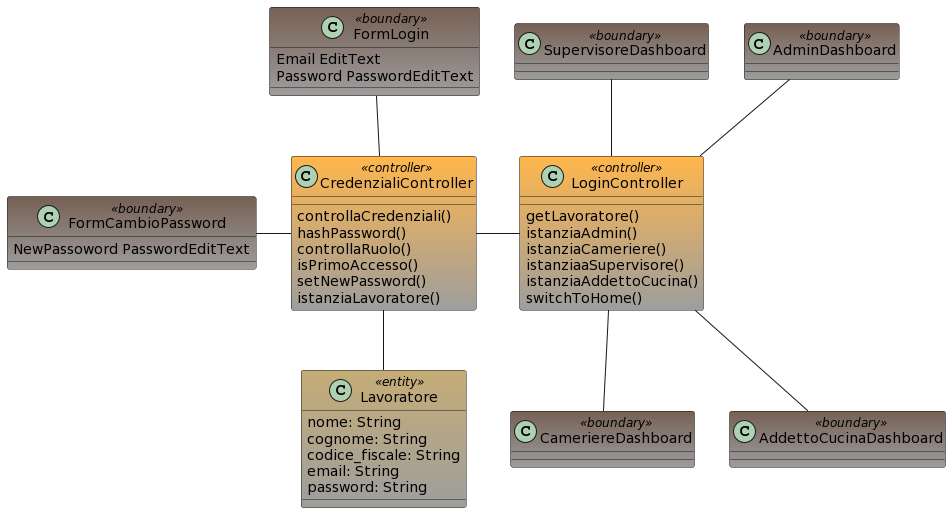
\includegraphics[scale=0.5]{assets/diagrammi/Class diagram di analisi/Login_3.png}
            \caption{\textbf{C01}: Class diagram Login}\label{fig:Login}
        \end{figure}

    \subsubsection{Class diagram Ristorante}
        \begin{figure}[H]
            \centering
            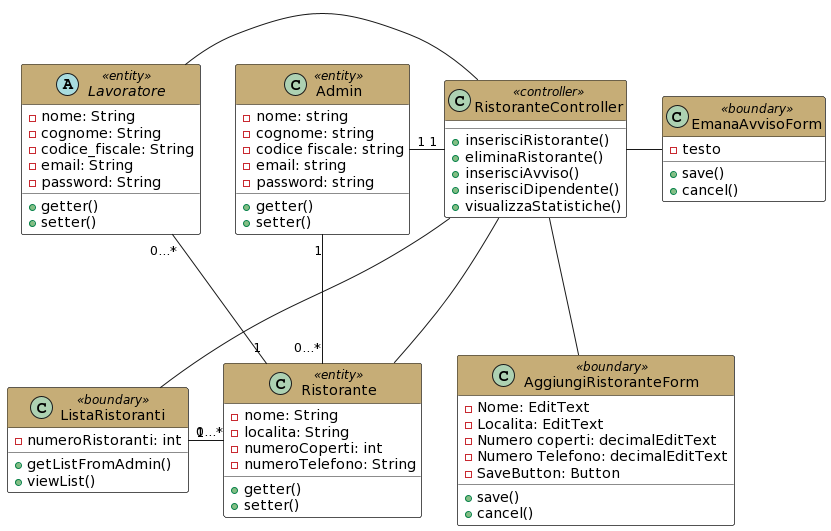
\includegraphics[scale=0.5]{assets/diagrammi/Class diagram di analisi/Gestione ristorante.png}
            \caption{\textbf{C02}: Class diagram Gestione ristorante}\label{fig:Ristorante}
        \end{figure}

    \subsubsection{Class diagram dipendenti}
        \begin{figure}[H]
            \centering
            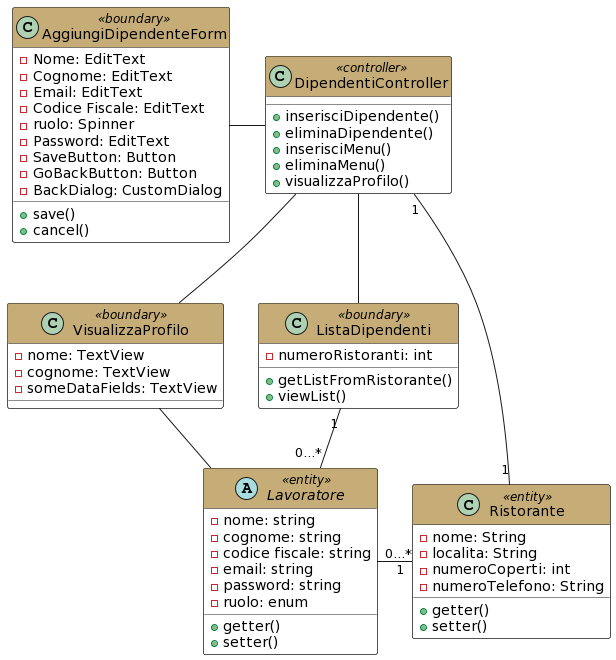
\includegraphics[scale=0.5]{assets/diagrammi/Class diagram di analisi/Gestione dipendenti.png}
            \caption{\textbf{C03}: Class diagram gestione dipendenti}\label{fig:Dipendenti}
        \end{figure}
    
    \subsubsection{Class diagram Menu}
        \begin{figure}[H]
            \centering
            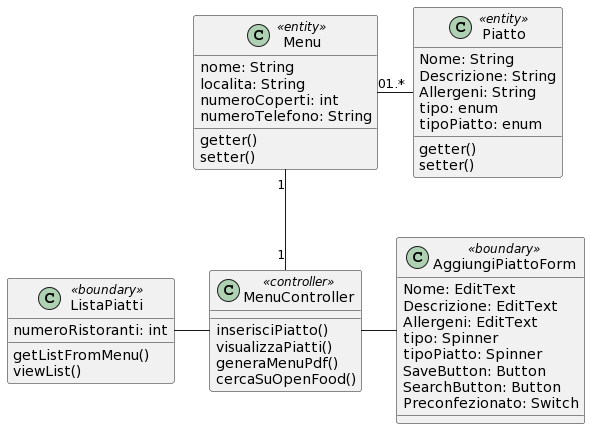
\includegraphics[scale=0.5]{assets/diagrammi/Class diagram di analisi/Gestione menu.png}
            \caption{\textbf{C04}: Class diagram gestione menu}\label{fig:Menu}
        \end{figure} 

    \subsubsection{Class diagram Avvisi}
        \begin{figure}[H]
            \centering
            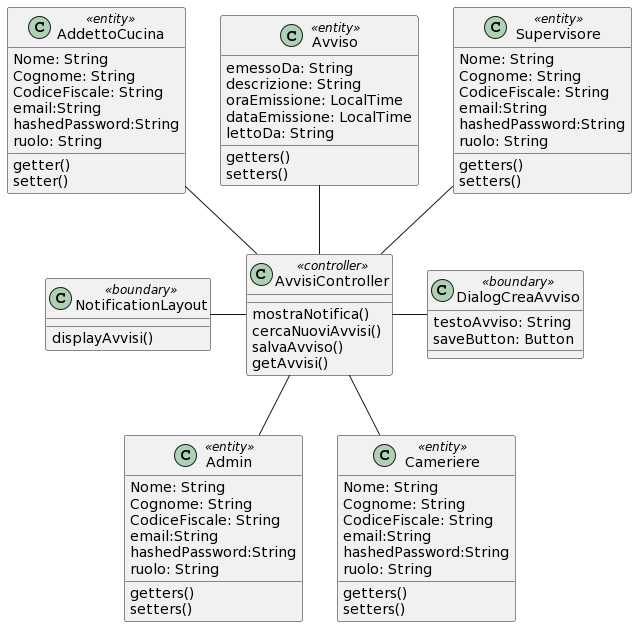
\includegraphics[scale=0.5]{assets/diagrammi/Class diagram di analisi/Gestione Avvisi.png}
            \caption{\textbf{C05}: Class diagram gestione avvisi}\label{fig:Avvisi}
        \end{figure}

    \subsubsection{Class diagram Ordini}
        \begin{figure}[H]
            \centering
            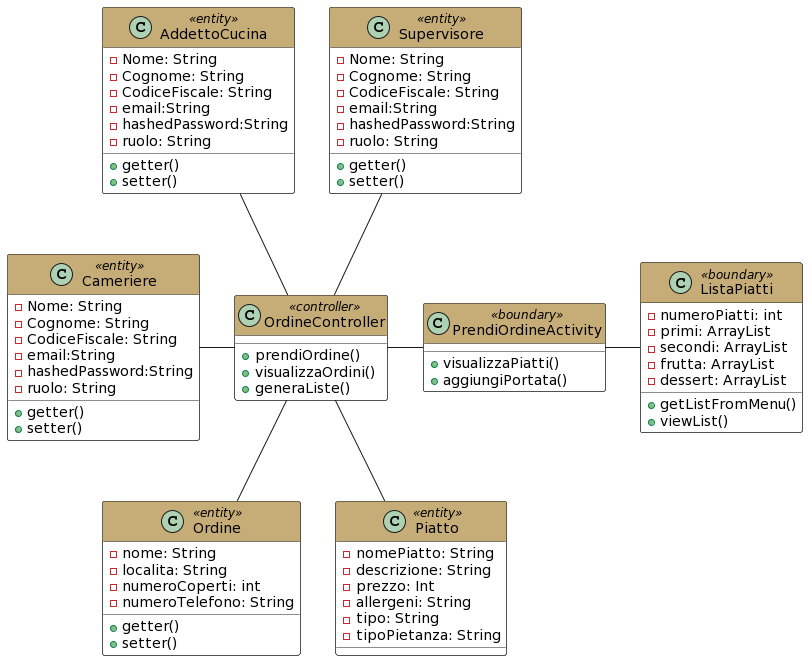
\includegraphics[scale=0.5]{assets/diagrammi/Class diagram di analisi/Gestione ordini.png}
            \caption{\textbf{C06}: Class diagram gestione ordini}\label{fig:Ordini}
        \end{figure}

    \subsubsection{Class diagram statistiche}
        \begin{figure}[H]
            \centering
            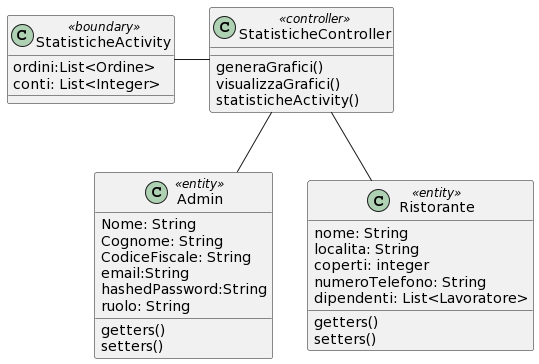
\includegraphics[scale=0.5]{assets/diagrammi/Class diagram di analisi/Gestione Stat.png}
            \caption{\textbf{C07}: Class diaram gestione statistiche}\label{fig:Statistiche}
        \end{figure}
    \subsection{Sequence di analisi}

    \begin{flushleft}
        Abbiamo scelto di modellare (in fase di analisi dei requisiti) con i sequence diagram i segenti casi d'uso:
        \begin{itemize}
            \item  \emph{Aggiunta menu del ristorante}
            \item  \emph{Prendere oridinazione}
        \end{itemize}
    \end{flushleft}
    \subsection{Prototipazione funzionale via statechart dell’interfaccia grafica}
    \begin{flushleft}
        Gli statechart sono uno strumento
        di modellazione grafica, utile per rappresentare il funzionamento di un
        sistema. Sono caratterizzati da stati e transizioni, che rappresentano il
        passaggio tra stati diversi. Sono inoltre molto importanti poichè forniscono
        un chiaro mezzo di costruzione di prototipi statici: con pochi semplici
        simboli è possibile modellare l'intero funzionamento di un'interfaccia grafica.
        Useremo questo potente strumento per rappresentare i seguenti casi d'uso:
        \emph{\textbf{Aggiungi ristorante}}, \emph{\textbf{Aggiungi piatto}}, 
        \emph{\textbf{Prendi ordine}} e \emph{\textbf{Visualizza avvisi}}. 
    \end{flushleft}

    \subsubsection{Aggiungi ristorante}
        \begin{figure}[H]
            \centering
            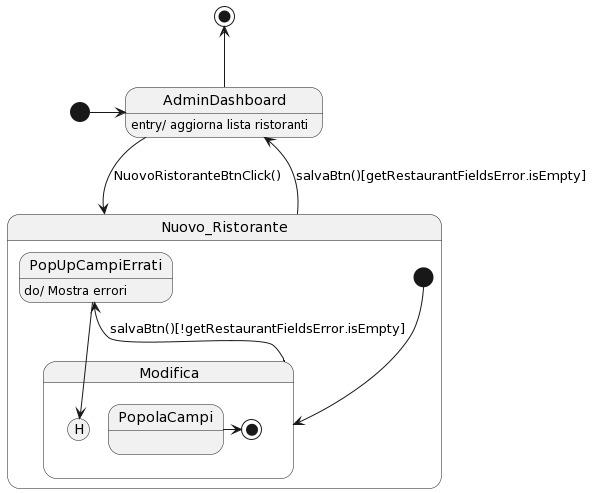
\includegraphics[scale=0.65]{assets/diagrammi/Statechart/aggiungiRistorante.png}
            \caption*{\textbf{Statechart} : aggiunta ristorante}\label{fig:Statechart_AddResturant}
        \end{figure}

    \subsubsection{Aggiungi piatto}
        \begin{figure}[H]
            \centering
            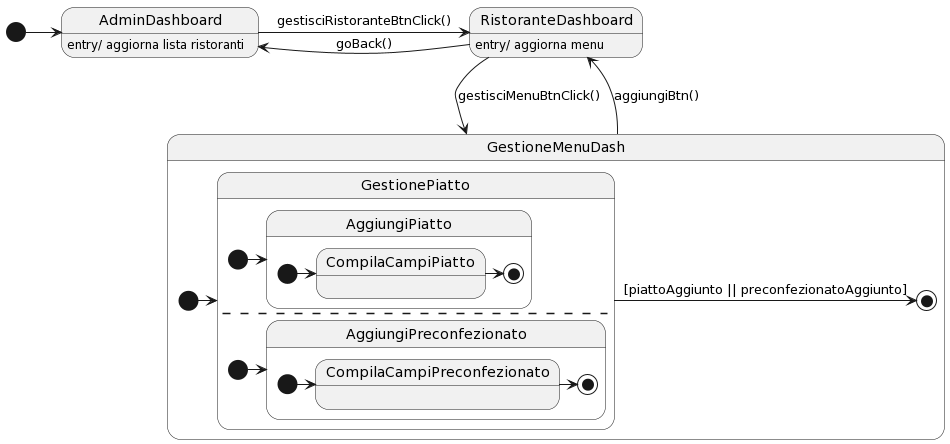
\includegraphics[scale=0.45]{assets/diagrammi/Statechart/aggiungiPiatto.png}
            \caption*{\textbf{Statechart} : aggiunta piatto}\label{fig:Statechart_AddPlate}
        \end{figure}

        \begin{figure}[H]
            \centering
            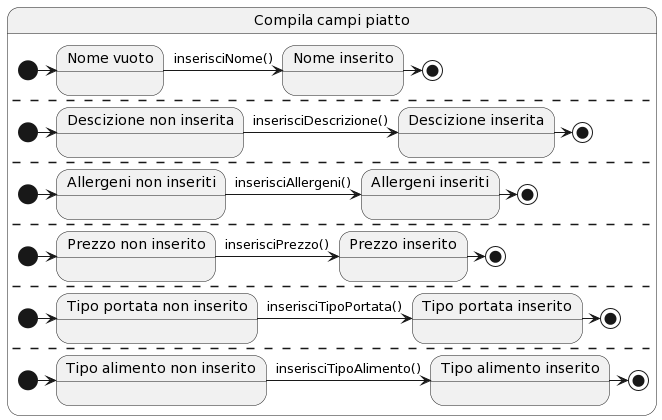
\includegraphics[scale=0.6]{assets/diagrammi/Statechart/compilaCampiPiatto.png}
            \caption*{\textbf{Statechart} : compilazione campi piatto non preconfezionato}\label{fig:Statechart_fieldPlate}
        \end{figure}

        \begin{figure}[H]
            \centering
            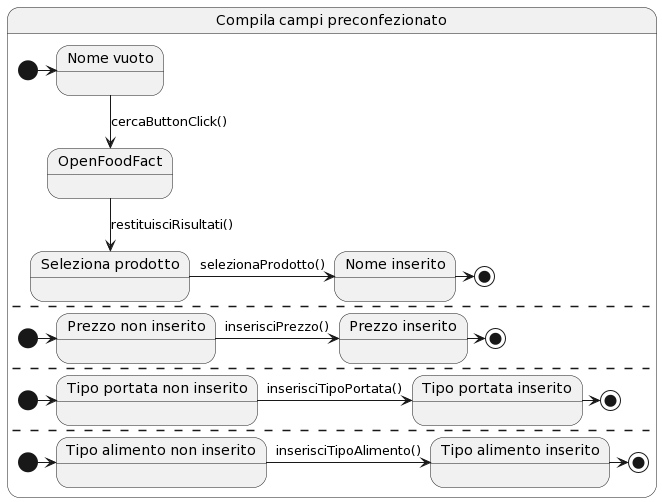
\includegraphics[scale=0.6]{assets/diagrammi/Statechart/compilaCampiPreconfezionato.png}
            \caption*{\textbf{Statechart} : compilazione campi piatto preconfezionato}\label{fig:Statechart_fieldPlate2}
        \end{figure}

    \subsubsection{Prendi ordine}
        \begin{figure}[H]
            \centering
            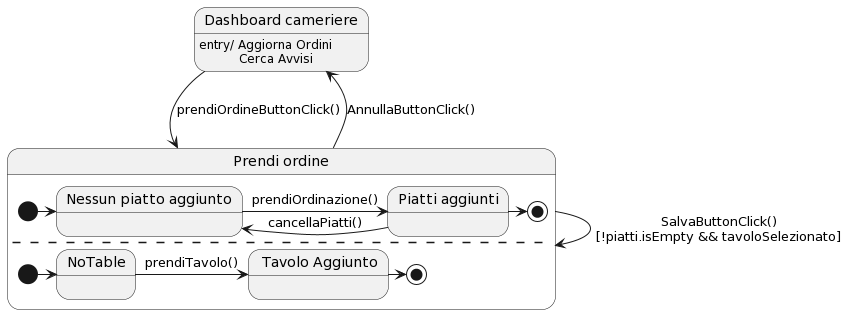
\includegraphics[scale=0.7]{assets/diagrammi/Statechart/prendiOrdine.png}
            \caption*{\textbf{Statechart} : Prendi ordinazione}\label{fig:Statechart_takeOrder}
        \end{figure}

    \subsubsection{Visualizza avvisi}
        \begin{figure}[H]
            \centering
            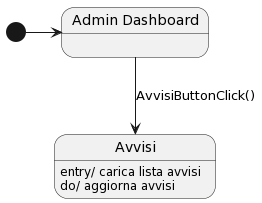
\includegraphics[scale=1]{assets/diagrammi/Statechart/visualizzaAvvisi.png}
            \caption*{\textbf{Statechart} : visualizzazione avvisi}\label{fig:Statechart_viewAdv}
        \end{figure}
    \section{Documento di design}
    \subsection{Architettura del sistema}

    \begin{flushleft}
        Alla luce delle valutazioni effettuate durante l'analisi dei requisiti, abbiamo trovato conveniente strutturare la nostra app seguendo un tipo di 
        architettura generale client-server (con server centralizzato). I client, nel nostro caso, sono quasi sempre dei dispositivi portatili dotati di sistema operativo android (con la possibilità volendo di utilizzare emulatori da pc desktop)
        mentre il server è stato realizzato con il framework di sviluppo Spring Boot. Il client comunica con il server che offre delle REST API attraverso delle richieste HTTP (le risposte del server saranno quasi sempre in formato JSON). 

    \end{flushleft}

    \subsubsection{Client}
    \begin{flushleft}
        Come già detto, il client è composto da un'applicazione android distribuita o tramite apk o tramite play store (rispetta tutti i requisiti per essere pubblicata) che mira ad offrire un'interfaccia utente semplice e pulita 
        per l'accesso agli endpoint forniti dal nostro server Spring-Boot. \\
        In generale, l'architettura di un progetto Android di default segue il pattern architetturale \emph{Model-View-Controller (MVC)}, 
        ma con alcune modifiche per adattarsi al contesto specifico di Android. In aggiunta, elenchiamo qui altri pattern e librerie che abbiamo adoperato per lo sviluppo dell'app:\\
        \vspace{1cm}
        \textbf{\emph{Pattern Singleton:}} Abbiamo usato il pattern Singleton per generare una sola istanza del dipendente che si logga nell'app. 
        Cosi facendo, è risultato più semplice aggiornare gli oggetti entità quali Cameriere, Addetto Cucina, Admin e Supervisore e mantenere costantemente un rapporto 1:1 con quanto salvato nel server.\vspace{1cm}
        
        \textbf{\emph{Pattern Observer:}} Molte componenti del sistema Android utilizzano il pattern Observer. 
        Il pattern Observer prevede che un oggetto, chiamato soggetto (Subject), mantenga una lista di oggetti dipendenti, chiamati osservatori (Observers), 
        e che questi vengano notificati automaticamente ogni volta che lo stato del soggetto cambia. In questo modo, 
        gli osservatori possono essere aggiornati in modo efficiente sullo stato del soggetto senza dover verificare continuamente se qualcosa è cambiato.
        In Android, il pattern Observer viene utilizzato, ad esempio, per gestire gli eventi generati dall'utente (come i tap sullo schermo), per notificare i cambiamenti nei dati  o per gestire la comunicazione tra componenti diversi dell'applicazione.
        Anche l'implementazione di \textbf{CallBack} come nel nostro caso (con VolleyCallback) possono essere viste come un' implementazione del pattern Observer.
        Più in particolare la nostra VolleyCallback, che altro non è che un'interfaccia, richiede di implementare in ogni Activity il metodo onResponse() che aggiorna i dati locali con i dati ricevuti dal server.
        Ciò che andiamo ad aggiornare in locale sono poi i Singleton del lavoratore loggato. Da lì, si passa poi all'aggiornamento delle viste nel caso di novità nell'oggetto risposta ricevuto. \vspace{1cm}
       
        \textbf{Volley} Volley è una libreria Android sviluppata da Google che semplifica l'elaborazione di richieste di rete in applicazioni Android. È stata progettata per gestire facilmente le chiamate REST API e può essere utilizzata per inviare e ricevere dati in diversi formati, come JSON, XML e immagini.
        Volley utilizza una combinazione di caching e pooling di connessioni per garantire prestazioni elevate e ridurre il consumo di risorse. Inoltre, supporta la gestione automatica di thread e gestisce in modo trasparente gli errori di rete, semplificando notevolmente la scrittura di codice robusto e affidabile.
        Implementata come Singleton, garantisce l'esistenza di una sola istanza di essa, e ci assicura consumi di memoria costanti e limitati.
        
        \textbf{Gson} Gson è una libreria Java sviluppata da Google che permette la serializzazione e la deserializzazione di oggetti JSON (JavaScript Object Notation) in oggetti Java. Gson offre una serie di metodi per la conversione di oggetti Java in JSON e viceversa, semplificando il processo di scambio di dati tra applicazioni Java e servizi web che utilizzano il formato JSON. 
    \end{flushleft}
    \vspace{0.2cm}


    \subsubsection{Server}
    \begin{flushleft}
        Il back-end della nostra applicazione è stato realizzato con la tecnlogia offerta da Spring Boot, un potente framework di svillupo che sfrutta Java.
        L'architettura che prevede è anch'essa a 3 livelli e prevede i seguenti componenti:
        \begin{itemize}
            \item Model: L'insieme di classi che rappresentano le entità della nostra applicazione. Le stesse sono riportate sul client, e, cosa più importate, spring mappa le classe con annotation "@entity" 1:1 con le tabelle nel db relazionale.\\
            \item Repository: Sfruttando il framework JPA (Java Persistence API) riusciamo a gestire persistenza e consistenza dei dati nel db in maniera quasi automatizzata. Spring ci fornisce un gran supporto in questo ambito.
            \item Controller: Qui ci va tutta la logica di controllo del server. Sono queste le classi che espongono gli end-point Rest ai client e, comunicando con le repository aggiornano i model e le tabelle nel db allo stesso tempo. Nel controller mappiamo tutti gli end-point a reindirizziamo le richieste http alla rispettiva funzione.
        \end{itemize}
    \end{flushleft}

    \begin{figure}[H]
        \centering
        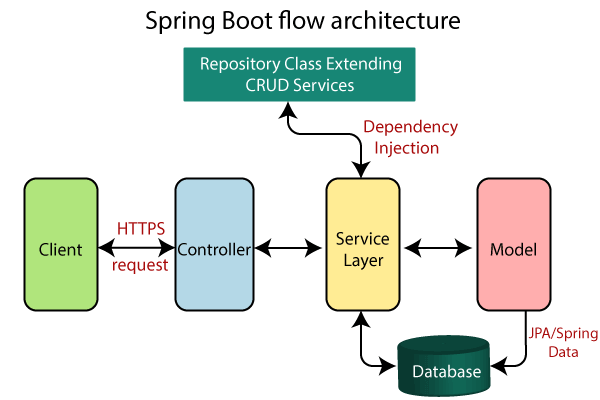
\includegraphics[scale=0.3]{assets/immagini varie/spring-boot-architecture2.png}
        \caption*{\textbf{Figura}: Spring-Boot}\label{fig:spring_Arch}
    \end{figure}

    \begin{flushleft}
        \textbf{Perchè Spring?}\\
        La scelta di utilizzare spring è dovuta principalmente alle sue caratteristiche di flessibilità e scalabilità. Semplifica inoltre lo sviluppo dell'intero applicativo
        grazie alle sue funzionalità di auto-configurazione e di gestione delle dipendenze, che avviene con Gradle e Maven. Spring Boot fornisce inoltre un'ampia gamma di funzionalità per sviluppare applicazioni web in modo rapido e facile. Queste funzionalità includono la gestione delle richieste HTTP, la gestione delle sessioni, la sicurezza, la gestione delle transazioni e, tra le altre, il pieno supporto alle API REST e operazioni CRUD.\\
        In sintesi, Spring Boot semplifica lo sviluppo di servizi web basati su REST e consente di creare API performanti, scalabili e sicure in modo rapido ed efficiente.
    \end{flushleft}
    

    \newpage

    \begin{flushleft}
        \textbf{Microsoft Azure}\\
        Microsoft Azure è la piattaforma cloud pubblica di Microsoft, che offre servizi di cloud computing. Tra i vari piani che mette a disposizione abbiamo usufruito
        di quello "gratuito" che ci ha permesso di eseguire una macchian virtuale linux (seppur con poche risorse) e un database relazionale, che nel nostro caso è stato PostgreSQL.
        La configurazione della macchina virtuale non ha richiesto particolari abilità: tramite connessione ssh abbiamo configurato il progetto Spring Boot e avviandolo 
        mettiamo a disposizione gli end-point raggiungibili poi dai client.
        La potenza computazionale in questa fase di sviluppo e di utilizzo limitato dell'applicativo potrebbe risultare esile, ma il vantaggio di piattaforme quali
        Azure è possibile in qualsiasi momento aumentare le risorse dedicate a db e/o macchina virtuale, aumentando di fatto la scalabilità della nostra applicazione.
    \end{flushleft}

    \begin{figure}[H]
        \centering
        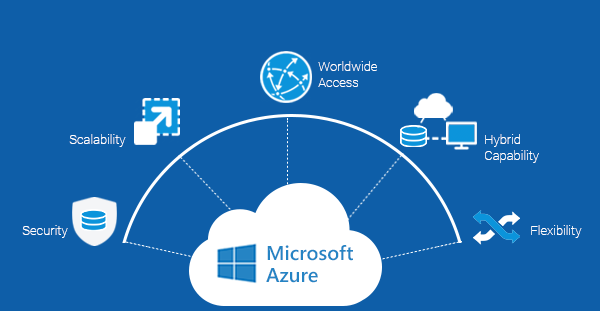
\includegraphics[scale=0.5]{assets/immagini varie/azure loc.png}
        \caption*{\textbf{Figura}: Micrsoft Azure}\label{fig:mic_az}
    \end{figure}
    \newpage
    \begin{flushleft}
        \textbf{E la sicurezza?}\\
        La sicurezza è garantita sia dalla sicurezza intrinseca dei servizi offerti da Microsoft Azure (parliamo quindi di operatività, assistenza, scalabilità) sia da un piccolo sistema di sicurezza pensato dal team:
    \end{flushleft}

    \begin{lstlisting}[language = Java, frame = trBL, firstnumber = last, escapeinside={(*@}{@*)}]
        @Component
        public class AppCodeInterceptor implements HandlerInterceptor {

            private static final String HEADER_APP_CODE = "app_code";
            private static final String EXPECTED_APP_CODE = "Ratatuille23";

            @Override
            public boolean preHandle(HttpServletRequest request, 
            HttpServletResponse response, Object handler) throws Exception {
                String appCode = request.getHeader(HEADER_APP_CODE);
                if (appCode == null || !appCode.equals(EXPECTED_APP_CODE)) {
                    System.out.println("Access denied");
                    response.setStatus(HttpStatus.UNAUTHORIZED.value());
                    return false;
                }
                return true;
            }
        }
    \end{lstlisting}
    

    \begin{flushleft}
        Questa piccola parte di codice presente nel back-end, ci garantisce che nessun'altra richiesta al di fuori da 
        quelle effettuate con il parametro "appcode" da noi definito sul client venga accettata.
        Estranei e malintenzionati, riceveranno lo status 401 se proveranno ad accedere a qualunque dei nostri endpoint.
    \end{flushleft}

   
        
    
    \subsection{Sequence diagram di design}

\subsubsection{Funzionalità: "Aggiungi Ristorante"}
\begin{flushleft}


\end{flushleft}


\begin{figure}[H]
    \centering
    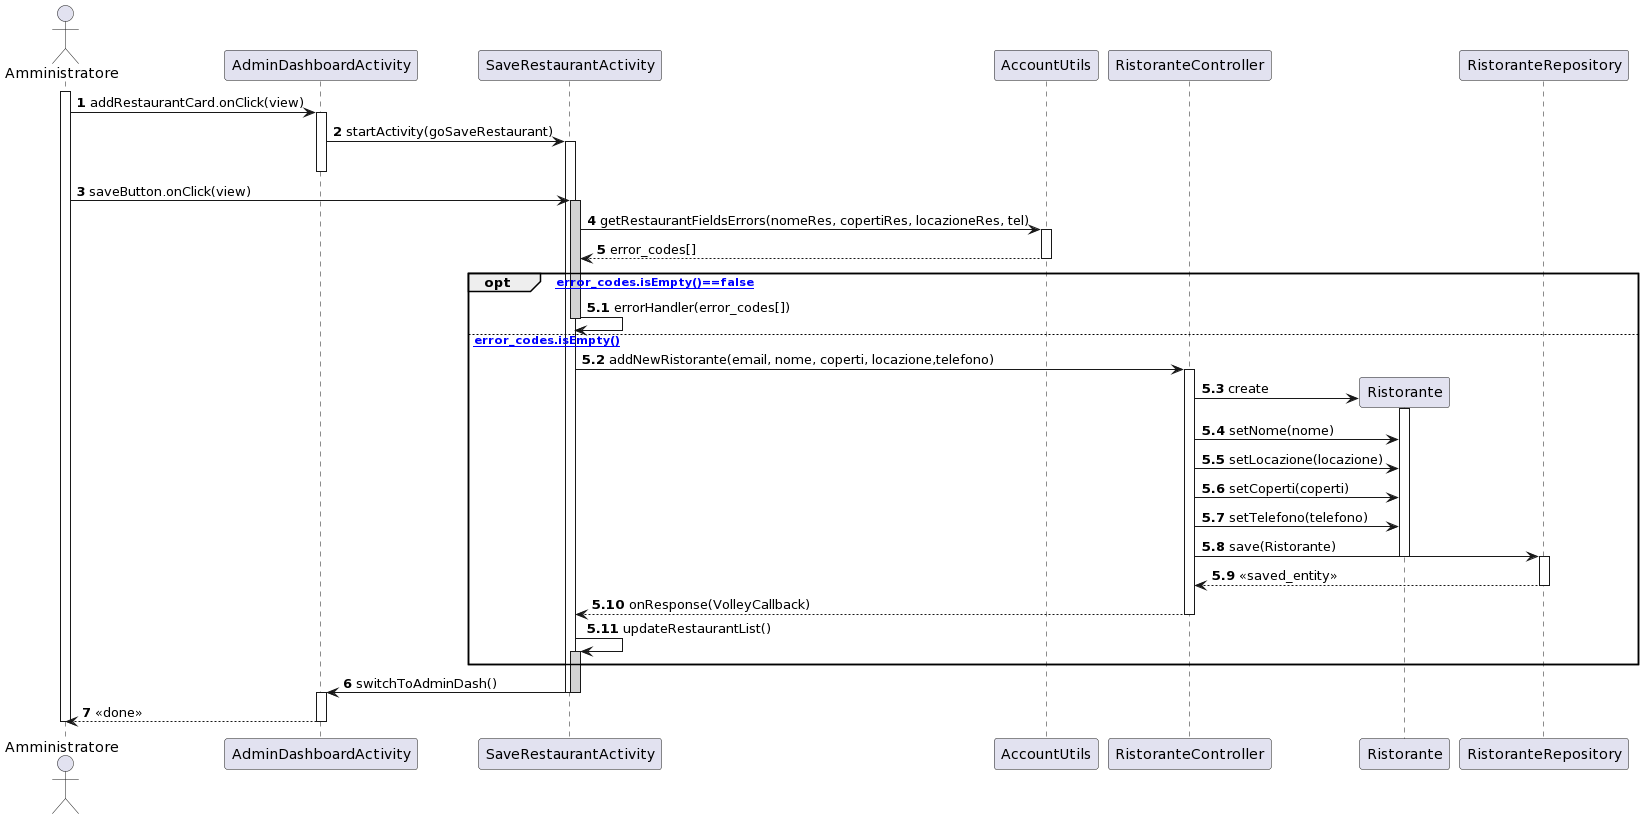
\includegraphics[scale=0.3]{assets/diagrammi/Sequence di design/Salva Ristorante.png}
    \caption{\textbf{Sequence}: Salva ristorante}\label{fig:seq_save_rest}
\end{figure}

\subsubsection{Funzionalità: "Aggiungi portata"}

\begin{figure}[H]
    \centering
    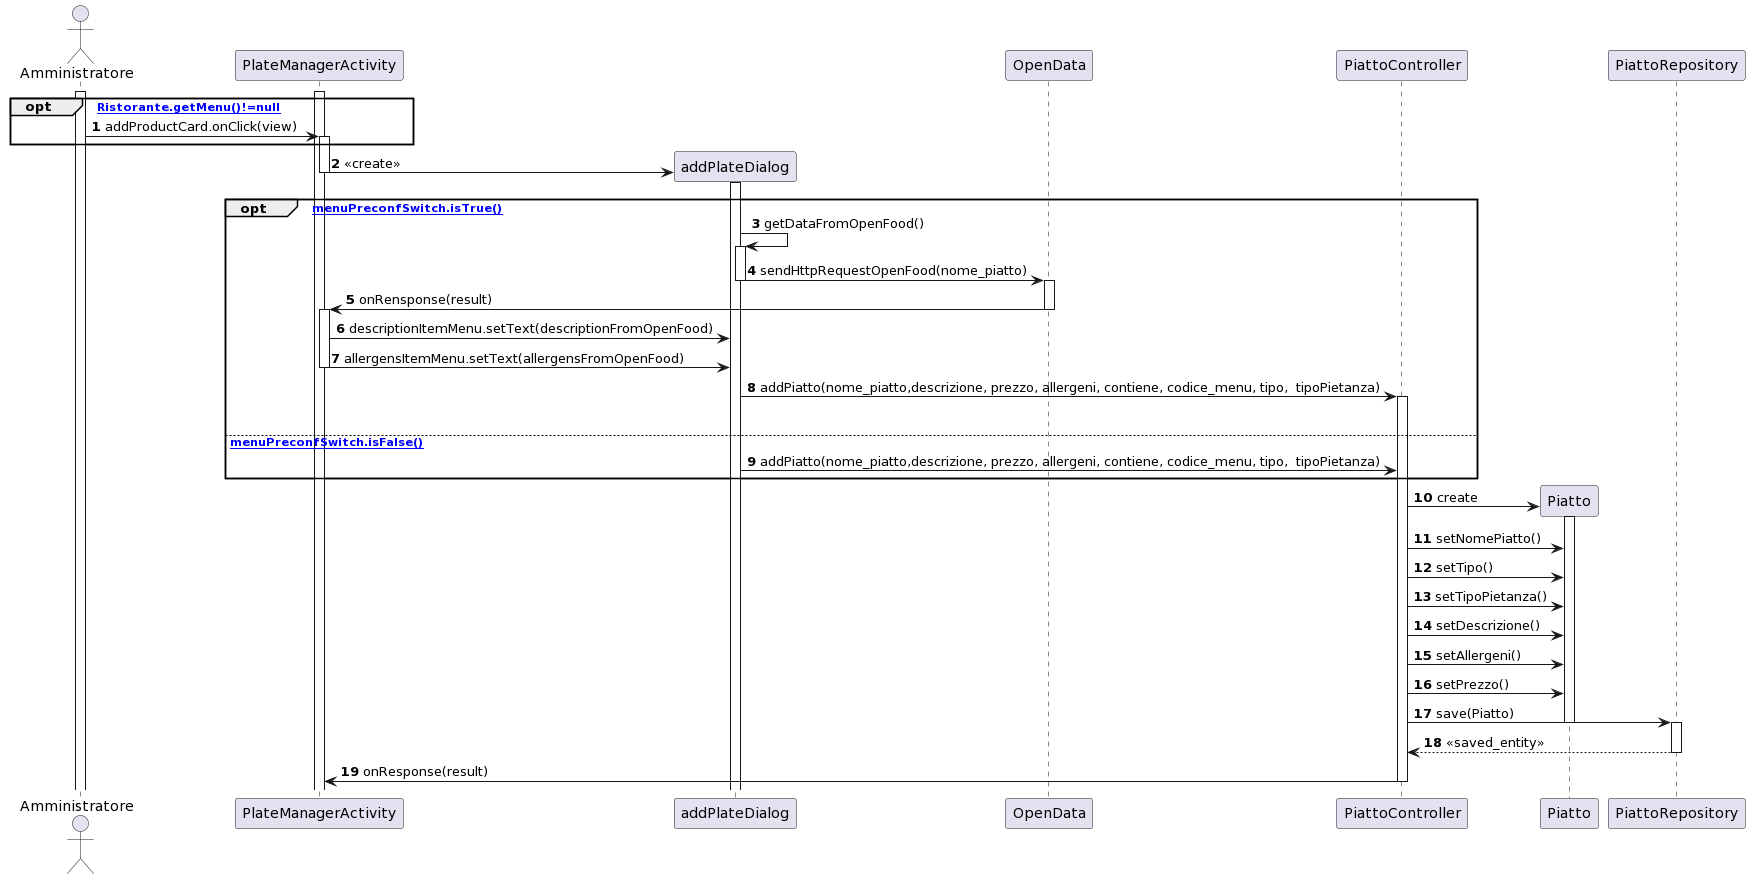
\includegraphics[scale=0.3]{assets/diagrammi/Sequence di design/Aggiungi Piatto.png}
    \caption{\textbf{Sequence}: Aggiunti portata}\label{fig:seq_save_plate}
\end{figure}
\newpage

\subsubsection{Funzionalità: "Prendi ordinazione"}
\subsubsection{Funzionalità: "Visualizza avvisi"}
\begin{figure}[H]
    \centering
    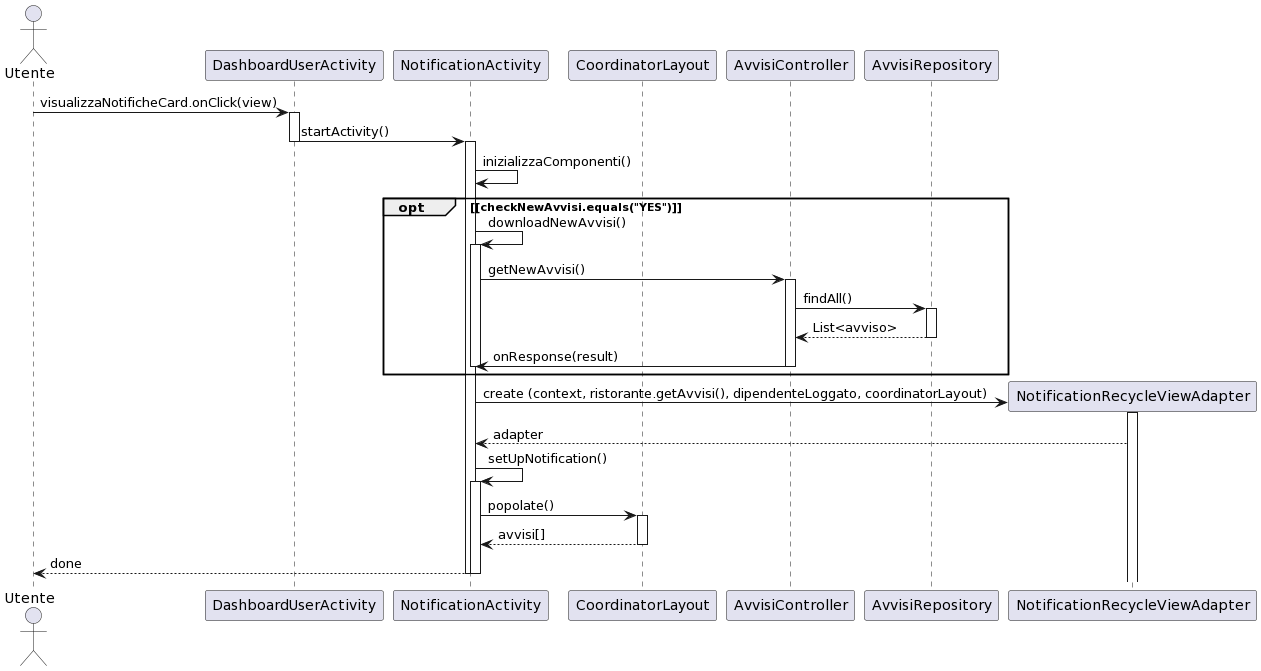
\includegraphics[scale=0.4]{assets/diagrammi/Sequence di design/Visualizza avvisi.png}
    \caption{\textbf{Sequence}: Visualizza avvisi}\label{fig:seq_view_avvisi}
\end{figure}

\newpage
    \subsection{Class diagram di design}
    \begin{flushleft}
        Verranno di seguito riportati i class diagram di design, che ora rispecchiano l'architettura del sistema e tutte le funzionalità nella loro
        interezza. \\
        \emph{\textbf{Nota}}: Tutti i costruttori banali (senza argomenti) e i getter e setter sono stati omessi per rendere più leggibili 
        i diagrammi
    \end{flushleft}

    \subsubsection{Login}
        \begin{figure}[H]
            \centering
            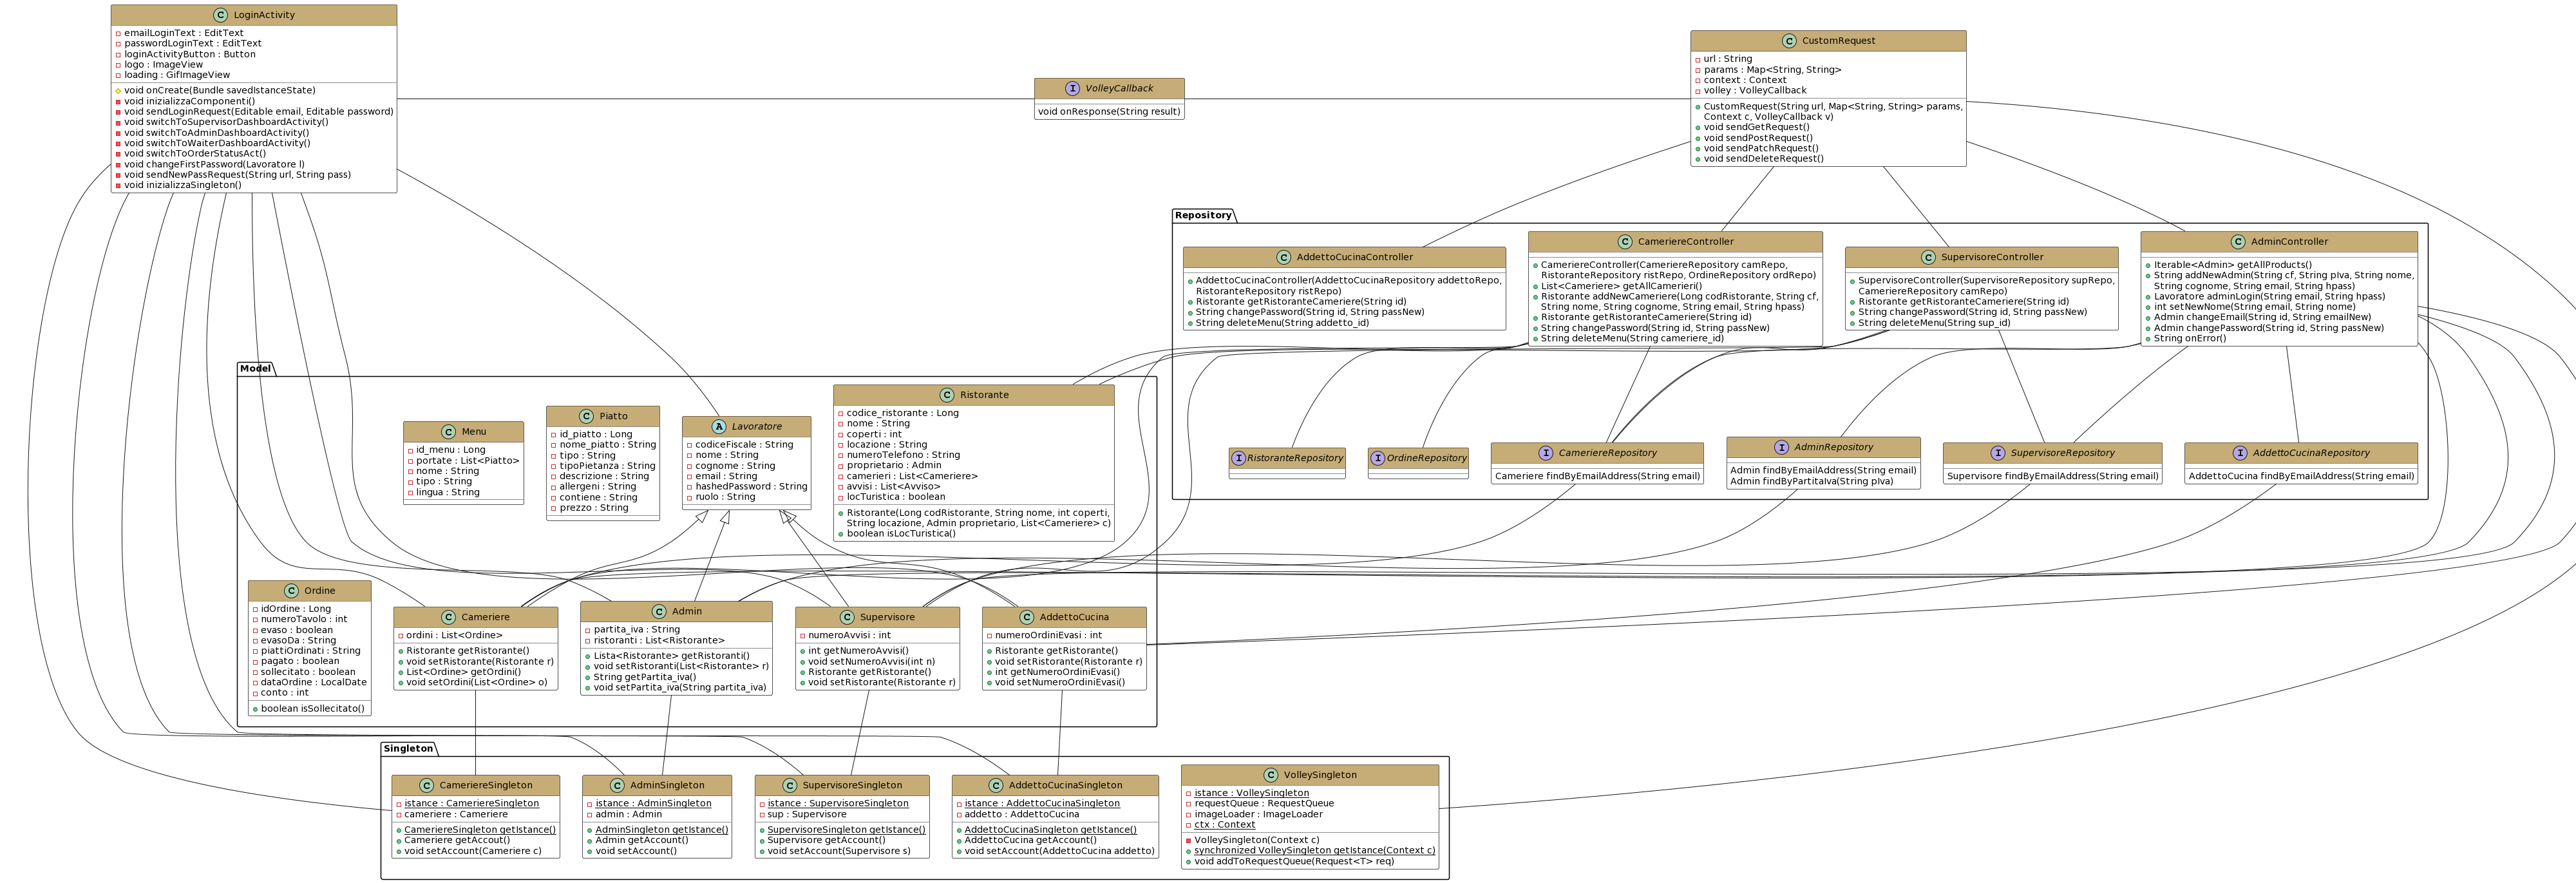
\includegraphics[scale=0.12]{assets/diagrammi/Class diagram di design/ClassDiagram_Login.png}
            \caption*{\textbf{CD01}: Class diagram Login}\label{fig:ClassDiagram_Login}
        \end{figure}
    
    \subsubsection{Gestione piatti}
        \begin{figure}[H]
            \centering
            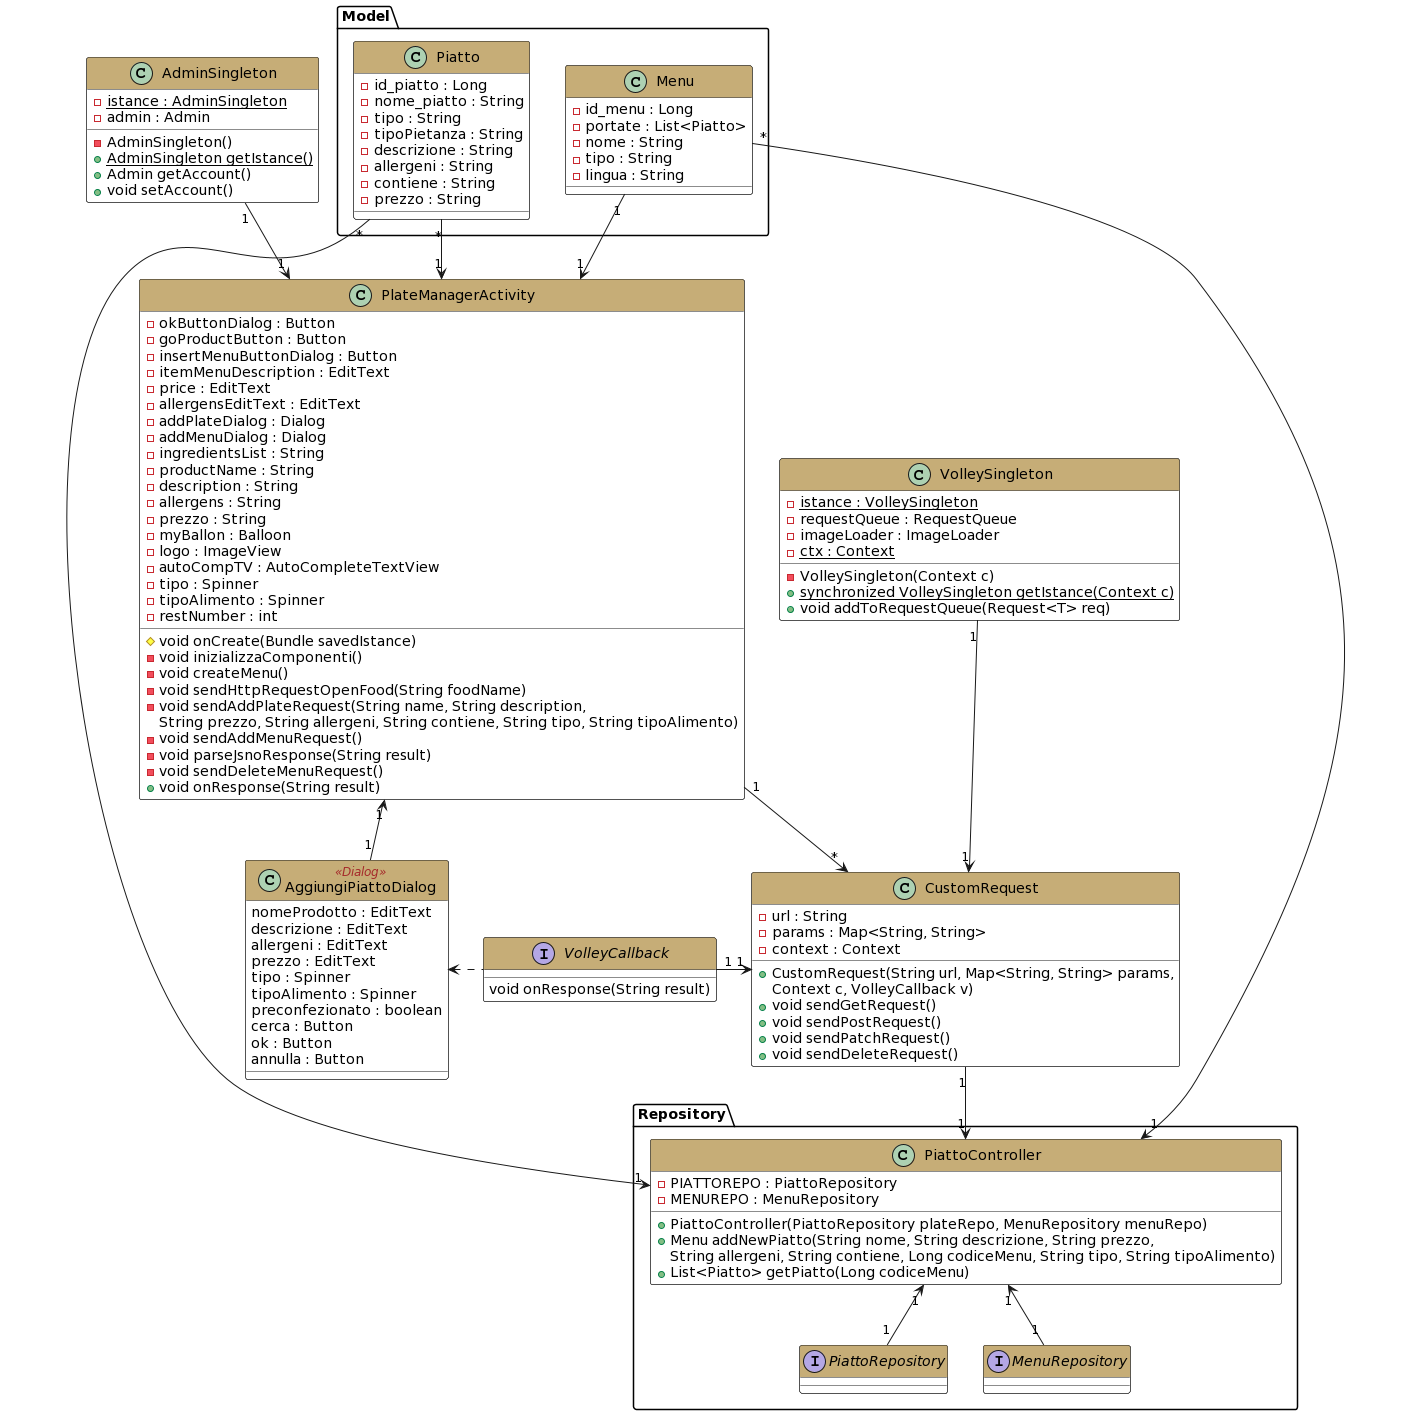
\includegraphics[scale=0.25]{assets/diagrammi/Class diagram di design/gestione piatti.png}
            \caption*{\textbf{CD02}: Class diagram gestione piatti}\label{fig:ClassDiagram_ManagePlates}
        \end{figure}

    \subsubsection{Gestione Avvisi}
        \begin{figure}[H]
            \centering
            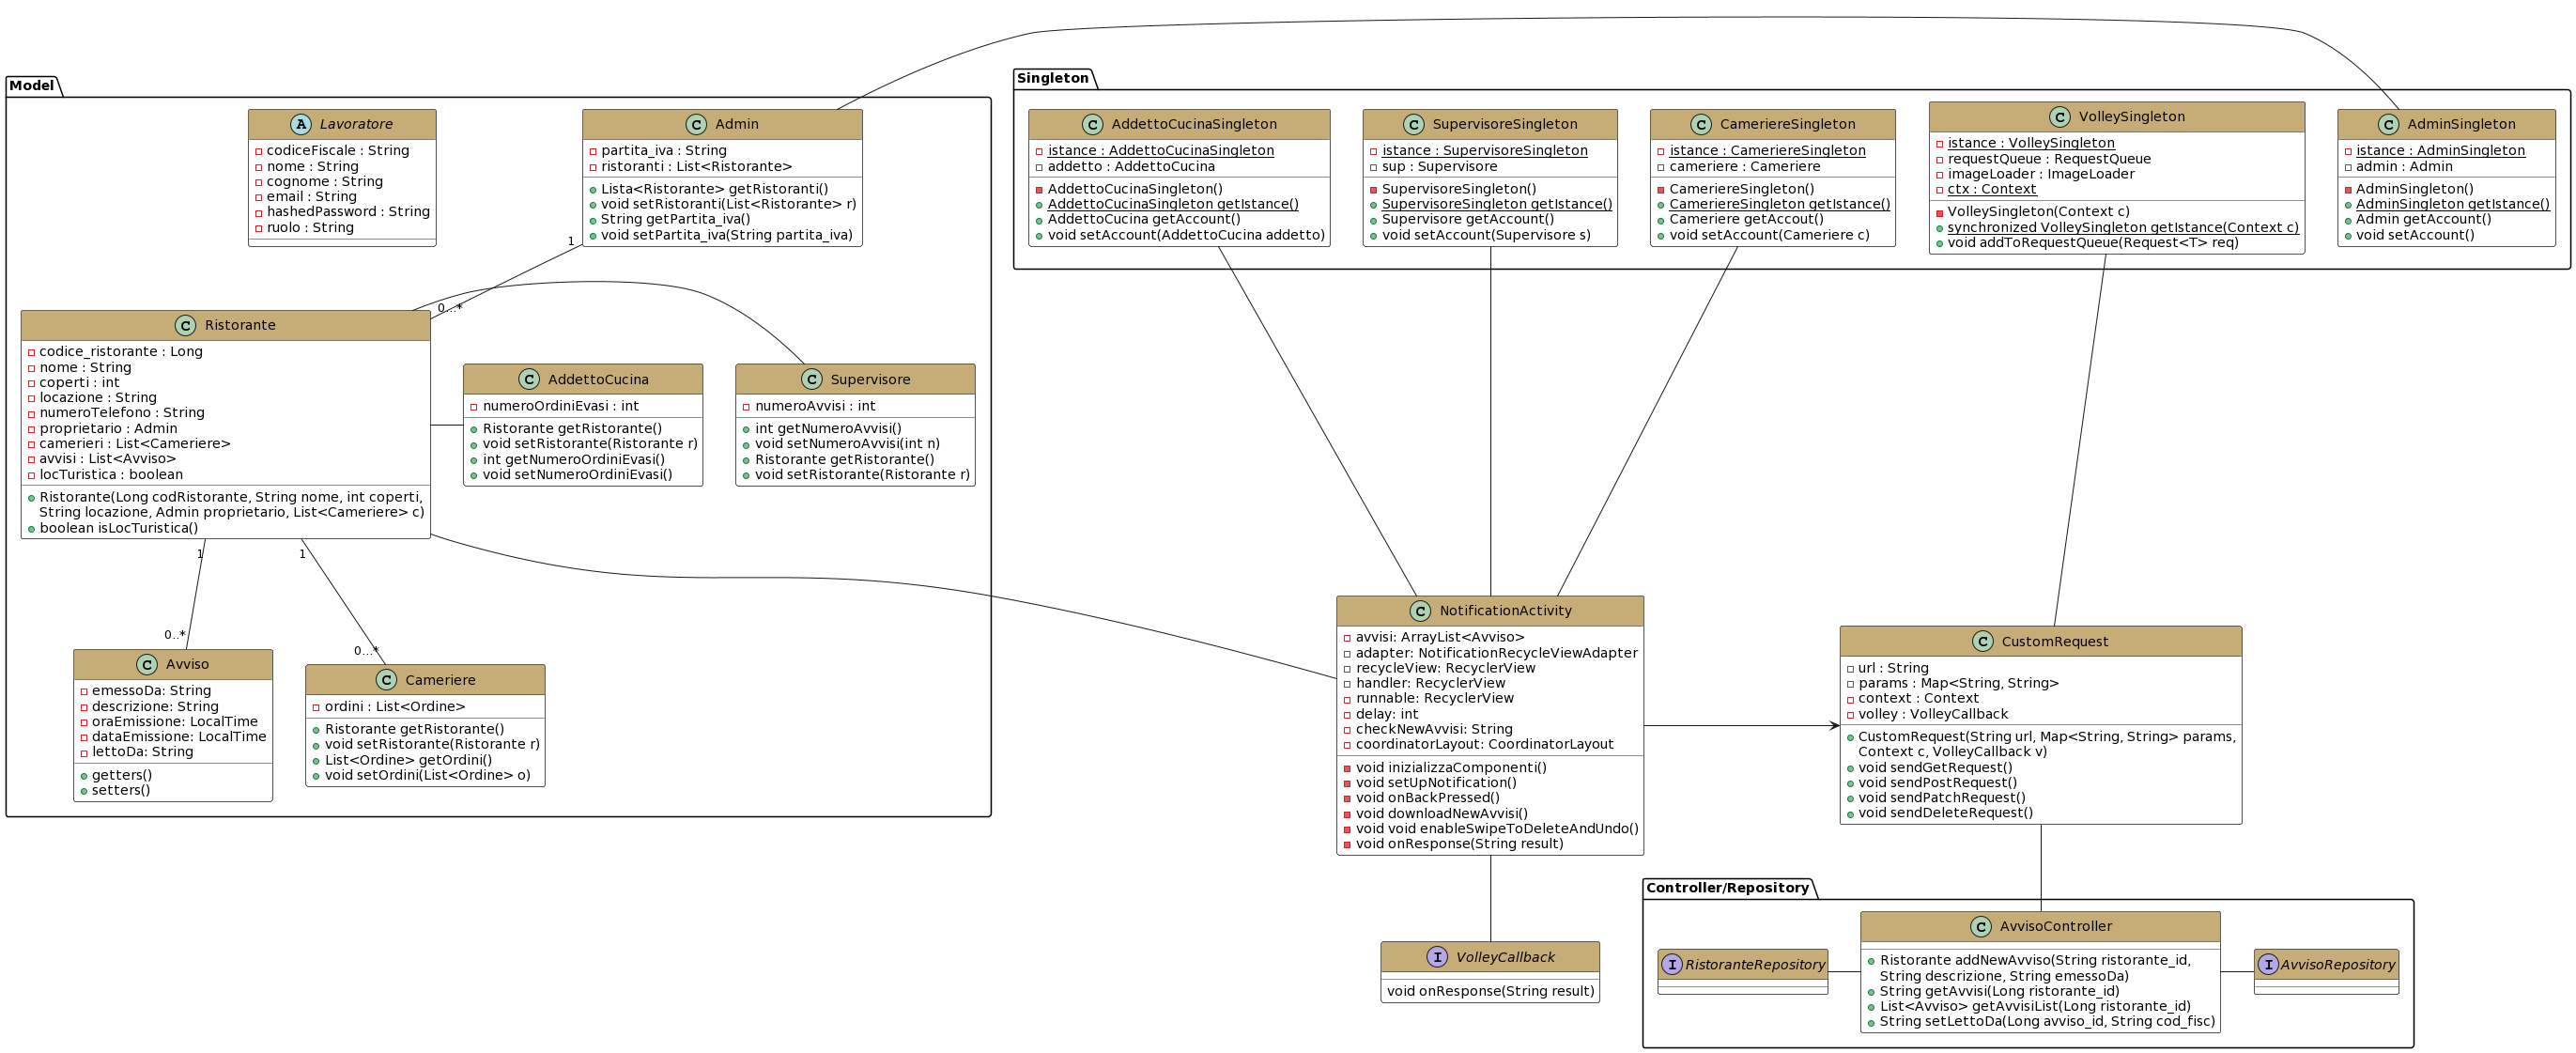
\includegraphics[scale=0.15]{assets/diagrammi/Class diagram di design/ClassDiagramGestioneAvvisi.png}
            \caption*{\textbf{CD03}: Class diagram gestione avvisi}\label{fig:ClassDiagram_ManageAdv}
        \end{figure}



    \section{Testing JUnit}

\lstset{
tabsize = 4, %% set tab space width
showstringspaces = false, %% prevent space marking in strings, string is defined as the text that is generally printed directly to the console
numbers = left, %% display line numbers on the left
commentstyle = \color{green}, %% set comment color
keywordstyle = \color{blue}, %% set keyword color
stringstyle = \color{red}, %% set string color
rulecolor = \color{black}, %% set frame color to avoid being affected by text color
basicstyle = \small \ttfamily, %% set listing font and size
breaklines = true, %% enable line breaking
numberstyle = \tiny,
}
 

\begin{flushleft}

    In questa sezione, presentiamo una delle fasi cruciali all'interno del ciclo di sviluppo del software, ovvero il testing. 
    Il testing può assumere diverse forme e tipologie, ma per la semplicità della presentazione, in questa sede si richiede
    il testing di soli 4 metodi con due o più parametri, che verrà effettuato mediante l'utilizzo del framework JUnit 5.
\end{flushleft}


%PRIMO METODO

\subsection{Test funzione check credenziali}
\begin{flushleft}
    
    Il metodo \textit{checkCredentials} ha il compito di verificare la validità di un indirizzo email
     e di una password. In particolare, il metodo accetta due stringhe come input: \textit{mail}, che 
     rappresenta l'indirizzo email, e \textit{pswrd}, che rappresenta la password.
    Il metodo restituisce un oggetto \textit{ArrayList} di interi, che rappresenta una 
    lista di eventuali errori verificatisi durante l'esecuzione del metodo. In altre parole, 
    il metodo controlla se l'indirizzo email e la password rispettano determinati requisiti, 
    e in caso contrario, aggiunge il corrispondente codice di errore alla lista.
    Infine, il metodo restituisce la lista degli errori, eventualmente vuota se non sono stati riscontrati problemi.\\
\end{flushleft}

\vspace{0.2cm}

\begin{lstlisting}[language = Java , frame = trBL , firstnumber = last , escapeinside={(*@}{@*)}, commentstyle=\color{brown}]

    public class CheckCredentialsTest {

    /*
    CLASSI DI EQUIVALENZA:
   
    PASSWORD: {VALIDA, VUOTA, TROPPO CORTA, NON RISPETTA LA REGEX}
      - VALIDA = Almeno 8 caratteri di cui 1 Maiuscola,
      1 Minuscola, 1 Carattere speciale, 1 numero

    EMAIL: {VALIDA, VUOTA, NON VALIDA}
      - VALIDA = Deve rispettare la sintassi
      di un email corretta

--------------------------------------------------------------------------------

    CODICI DI ERRORE:
      9 = PASSWORD VUOTA,
      10 = PASSWORD TROPPO CORTA,
      11 = PASSWORD NON VALIDA (REGEX)
      12 = EMAIL VUOTA, 
      13 = EMAIL NON VALIDA

---------------------------------------------------------------------------------

    STRATEGIE DI TESTING UTILIZZATE: 
      BlackBox secondo il criterio SECT

    CASI DI TESTING INDIVIDUATI: 
      22 in 12 metodi

------------------------------------------------------------------------------ */

    public ArrayList<Integer> codici_errore = new ArrayList<Integer>();

    @AfterEach
    public void clearArrayList() {
        codici_errore.clear();
    }

    @Test
    public void testCheckCredentials(){
        assertEquals(codici_errore, checkCredentials("ser.dimartino@studenti.unina.it", "Password.123"));
    }

    @Test
    public void tesPasswordVuota(){
        codici_errore.add(9);
        assertAll(
                () -> assertEquals(codici_errore, checkCredentials("fra.cutugno@studenti.unina.it", null)),
                () -> assertEquals(codici_errore, checkCredentials("lu.starace@studenti.unina.it", ""))
        );
    }

    @Test
    public void testPasswordTroppoCorta(){
        codici_errore.add(10);
        assertEquals(codici_errore, checkCredentials("gio.cutolo@studenti.unina.it", "Aa_09."));
    }

    @Test
    public void testPasswordNonValida(){
        codici_errore.add(11);
        assertAll(
                () -> assertEquals(codici_errore, checkCredentials("alb.aloisio@studenti.unina.it", "password?123")),  // MANCA LA MAIUSCOLA
                () -> assertEquals(codici_errore, checkCredentials("an.corazza@studenti.unina.it", "PASSWORD#123")),  //MANCA LA MINUSCOLA
                () -> assertEquals(codici_errore, checkCredentials("alb.aloisio@studenti.unina.it", "Password123")),  // MANCA IL CARATTERE SPECIALE
                () -> assertEquals(codici_errore, checkCredentials("an.corazza@studenti.unina.it", "Password_unoduetre")) // MANCA IL NUMERO
        );

    }

    @Test
    public void testEmailVuota(){
        codici_errore.add(12);
        assertAll(
                () -> assertEquals(codici_errore, checkCredentials(null, "Password.123")),
                () -> assertEquals(codici_errore, checkCredentials("", "Password.123"))
        );
    }

    @Test
    public void testEmaildNonValida(){
        codici_errore.add(13);
        assertAll(
                () -> assertEquals(codici_errore, checkCredentials("emailcompletamentesbagliata", "Password.123")),  // EMAIL COMPLETAMENTE SBAGLIATA
                () -> assertEquals(codici_errore, checkCredentials("@gmail.com", "Password.123")),  // MANCA LO USERNAME
                () -> assertEquals(codici_errore, checkCredentials("biagio@.net", "Password.123")),  // MANCA IL SECOND LEVEL DOMAIN
                () -> assertEquals(codici_errore, checkCredentials("matteo@libero.", "Password.123")), // MANCA IL TOP LEVEL DOMAIN
                () -> assertEquals(codici_errore, checkCredentials("luigivirgilio.it", "Password.123")), //MANCA LA @
                () -> assertEquals(codici_errore, checkCredentials("MATTEO[BIAGIO]LUIGI_@libero.IT", "Password.123")) // LO USERNAME PRESENTA CARATTERI NON CORRETTI
        );
    }

    @Test
    public void testErroriMultipli_9_12(){
        codici_errore.add(9);
        codici_errore.add(12);

        assertEquals(codici_errore, checkCredentials("", ""));
    }

    @Test
    public void testErroriMultipli_9_13(){
        codici_errore.add(9);
        codici_errore.add(13);

        assertEquals(codici_errore, checkCredentials("@studenti.@libero@com", ""));
    }

    @Test
    public void testErroriMultipli_10_12(){
        codici_errore.add(10);
        codici_errore.add(12);

        assertEquals(codici_errore, checkCredentials("", "Ab.34"));
    }

    @Test
    public void testErroriMultipli_10_13(){
        codici_errore.add(10);
        codici_errore.add(13);

        assertEquals(codici_errore, checkCredentials("emailcompletamentesbagliata", "Ab.34"));
    }

    @Test
    public void testErroriMultipli_11_12(){
        codici_errore.add(11);
        codici_errore.add(12);

        assertEquals(codici_errore, checkCredentials("", "Password.Password"));
    }

    @Test
    public void testErroriMultipli_11_13(){
        codici_errore.add(11);
        codici_errore.add(13);

        assertEquals(codici_errore, checkCredentials("@studenti.@libero@com", "@studenti.it"));
    }
}

\end{lstlisting}



%SECONDO METODO
\subsection{Test funzione che calcola incasso in un range di date.}
\begin{flushleft}
   La funzione "getIncassoRangeGiorni" prende in input una data di inizio e una lista di ordini e calcola l'incasso totale degli ordini che sono stati effettuati tra la data di inizio e la data attuale.

    La funzione controlla che la lista degli ordini non sia nulla. In caso contrario, restituisce zero. Successivamente, per ogni ordine nella lista degli ordini, la funzione controlla se la data dell'ordine è compresa tra la data di inizio e la data attuale. Se la data è compresa nel range, l'importo dell'ordine viene aggiunto all'incasso totale.
    
    Infine, la funzione restituisce l'incasso totale degli ordini effettuati nel range di tempo specificato.
\end{flushleft}
\vspace{0.2cm}

\begin{flushleft}
    Dato che la funzione "getIncassoRangeGiorni" fa parte della classe StatisticsActivity e fa uso della classe Ordini,
    abbiamo creato nel Package "Driver" i seguenti \textit{Mock} per poter eseguire il testing:
\end{flushleft}
\vspace{1cm}

\begin{lstlisting}[language = Java , frame = trBL , firstnumber = last , escapeinside={(*@}{@*)} , commentstyle=\color{brown}]
    public class StatisticsActivityMock {

    public float media(int giorni, float incasso){
        float media = 0;
        if(giorni < 0) throw new IllegalArgumentException("Il numero di giorni non deve essere negativo");
        if (giorni == 0) throw new ArithmeticException("Il numero di giorni non puo essere 0");
        if (incasso < 0) throw new IllegalArgumentException("l'incasso deve essere maggiore di 0.");
        media = incasso / giorni;
        media = Math.round(media * 100) / 100f;

        return media;
    }

    public int getIncassoRangeGiorni(LocalDate dataInizio, ArrayList<OrdineMock> orders){
        int incassoTotale = 0;
        LocalDate endDate = LocalDate.now();
        DateTimeFormatter formatter = DateTimeFormatter.ofPattern("yyyy-MM-dd");

        if (orders == null) return 0;
        for (OrdineMock ordine : orders) {
            LocalDate orderDate = LocalDate.parse(ordine.getDataOrdine(), formatter);
            if (orderDate.isEqual(dataInizio) || orderDate.isAfter(dataInizio) && orderDate.isBefore(endDate)) {
                incassoTotale += ordine.getConto();


            }
        }
        return incassoTotale;
    }
}
\end{lstlisting}
\vspace{0.2cm}

\begin{lstlisting}[language = Java , frame = trBL , firstnumber = last , escapeinside={(*@}{@*)} , commentstyle=\color{brown}]
   
 /*
    IN QUESTO CASO LA CLASSE ORDINE MOCK CONTIENE SOLO
    GLI ATTRIBUTI DI ORDINE CHE ENTRANO IN GIOCO ALL'INTERNO
    DEL METODO getIncassoRangeGiorni
*/

public class OrdineMock {

   private int conto;
   private String dataOrdine;

   public OrdineMock(int conto, String dataOrdine) {
       this.conto = conto;
       this.dataOrdine = dataOrdine;
   }

   public int getConto() {
       return conto;
   }

   public String getDataOrdine() {
       return dataOrdine;
   }
}

\end{lstlisting}
\vspace{0.2cm}
    
\begin{lstlisting}[language = Java , frame = trBL , firstnumber = last , escapeinside={(*@}{@*)} , commentstyle=\color{brown}]

/*
   CLASSI DI EQUIVALENZA:
   
      DATA_INIZIO: {VALIDA, NULL}
        - Valida: a sua volta puo' essere
             1.1) Verosimile e precedente agli ordini
             1.2) Futura agli ordini
             1.3) Inverosimilmente precedente agli ordini

      ORDINI: {VALIDI, NULL, LISTA VUOTA, CON DATA SBAGLIATA}

 --------------------------------------------------------------------------------

   STRATEGIE DI TESTING UTILIZZATE:

      BlackBox secondo il criterio WECT
      
   CASI DI TESTING RITENUTI NECESSARI:
     {VALIDA , VALIDI} : 1 Caso
     {VALIDA , NULL} : 1 Caso
     {VALIDA , LISTA VUOTA} : 1 Caso
     {VALIDA , CON DATA SBAGLIATA} : 4 Casi
     {DATA FUTURA , VALIDI} : 1 Caso
     {DATA INVEROSIMILMENTE PRECEDENTE , VALIDI} : 1 Caso
     {NULL , VALIDI} : 1 Caso

 ------------------------------------------------------------------------------ */  

public class getIncassoRangeGiorniTest {

    StatisticsActivityMock statisticsActivityMock;
    ArrayList<OrdineMock> ordiniM;
    DateTimeFormatter formatter;

    @Before
    public void setUp(){
        statisticsActivityMock = new StatisticsActivityMock();
        ordiniM = new ArrayList<>();
        formatter = DateTimeFormatter.ofPattern("yyyy-MM-dd");
    }

    @AfterEach
    public void clearArrayList(){
        ordiniM.clear();
    }


    @Test
    public void testGetIncassoRangeGiorni() {
        ordiniM.add(new OrdineMock(3, "2023-05-04"));
        ordiniM.add(new OrdineMock(105, "2023-05-04"));
        ordiniM.add(new OrdineMock(72, "2023-02-04"));

        LocalDate dataInizio = LocalDate.parse("2023-02-05", formatter);

        int result = statisticsActivityMock.getIncassoRangeGiorni(dataInizio, ordiniM);
        assertEquals(108, result);
    }

    @Test
    public void testZeroOrdini()  {
        LocalDate dataInizio = LocalDate.parse("2023-02-01", formatter);

        int result = statisticsActivityMock.getIncassoRangeGiorni(dataInizio, ordiniM);
        assertEquals(0, result);

    }

    @Test
    public void testOrdiniNull()  {
        LocalDate dataInizio = LocalDate.parse("2023-02-01", formatter);

        int result = statisticsActivityMock.getIncassoRangeGiorni(dataInizio, null);
        assertEquals(0, result);

    }

    @Test
    public void testDataInizioNull()  {
        ordiniM.add(new OrdineMock(3, "2023-05-04"));
        ordiniM.add(new OrdineMock(105, "2023-05-04"));
        ordiniM.add(new OrdineMock(72, "2023-02-04"));

        assertThrows(NullPointerException.class,
                () -> statisticsActivityMock.getIncassoRangeGiorni(null, ordiniM));
    }

    @Test
    public void testDataInizioFutura() {
        ordiniM.add(new OrdineMock(3, "2023-05-04"));
        ordiniM.add(new OrdineMock(105, "2023-05-04"));
        ordiniM.add(new OrdineMock(72, "2023-02-04"));

        LocalDate dataInizio = LocalDate.parse("2033-02-05", formatter);

        int result = statisticsActivityMock.getIncassoRangeGiorni(dataInizio, ordiniM);
        assertEquals(0, result);
    }

    @Test
    public void testDataInizioIrrealistica() {
        ordiniM.add(new OrdineMock(3, "2023-05-04"));
        ordiniM.add(new OrdineMock(105, "2023-05-04"));
        ordiniM.add(new OrdineMock(72, "2023-02-04"));

        LocalDate dataInizio = LocalDate.parse("0133-02-05", formatter);

        int result = statisticsActivityMock.getIncassoRangeGiorni(dataInizio, ordiniM);
        assertEquals(180, result);
    }

    @Test
    public void testDataOrdiniInFormatoSbagliato(){
        ArrayList<OrdineMock> ordiniM_1 = new ArrayList<>();
        ArrayList<OrdineMock> ordiniM_2 = new ArrayList<>();
        ArrayList<OrdineMock> ordiniM_3 = new ArrayList<>();
        ArrayList<OrdineMock> ordiniM_4 = new ArrayList<>();

        ordiniM_1.add(new OrdineMock(3, "2023"));
        ordiniM_2.add(new OrdineMock(105, "02/05/2023"));
        ordiniM_3.add(new OrdineMock(72, "due-aprile-2023"));
        ordiniM_4.add(new OrdineMock(105, "2023-32-31"));


        LocalDate dataInizio = LocalDate.parse("2023-02-01", formatter);

        assertAll(
                () ->   assertThrows(DateTimeParseException.class,
                        () -> statisticsActivityMock.getIncassoRangeGiorni(dataInizio, ordiniM_1)
                ),
                () ->   assertThrows(DateTimeParseException.class,
                        () ->statisticsActivityMock.getIncassoRangeGiorni(dataInizio, ordiniM_2)
                ),
                () ->   assertThrows(DateTimeParseException.class,
                        () -> statisticsActivityMock.getIncassoRangeGiorni(dataInizio, ordiniM_3)
                ),
                () ->   assertThrows(DateTimeException.class,
                        () -> statisticsActivityMock.getIncassoRangeGiorni(dataInizio, ordiniM_4)
                )

        );
        ordiniM_1.clear();
        ordiniM_2.clear();
        ordiniM_3.clear();
        ordiniM_4.clear();
    }

}

\end{lstlisting}


%TERZO METODO

\subsection{Test funzione che controlla i campi di un ristorante.}
\begin{flushleft}
    Questo metodo prende in input quattro stringhe che rappresentano il nome di un ristorante,
     il numero di coperti, l'indirizzo' e il numero di telefono. Il metodo restituisce un oggetto ArrayList
     di interi che rappresenta una lista di eventuali errori verificatisi durante l'esecuzione del metodo.
\end{flushleft}
\vspace{0.2cm}

\begin{lstlisting}[language = Java , frame = trBL , firstnumber = last , escapeinside={(*@}{@*)} , commentstyle=\color{brown}]
public class getRestaurantFiedlsErrorsTest {
/*
    CLASSI DI EQUIVALENZA:
 
       NOME: {VALIDO, VUOTO, TROPPO CORTO}
 
       COPERTI: {VALIDO, VUOTO, FUORI-RANGE, NON VALIDO}
         - FUORI RANGE: <5 && > 1000
         - NON VALIDO: Non composto da soli numeri
 
       INDIRIZZO: {VALIDO, VUOTO, TROPPO CORTO, NON VALIDO}
         - NON VALIDO: Contiene caratteri speciali
 
       TELEFONO: {VALIDO, VUOTO, NON VALIDO}
 
  --------------------------------------------------------------------------------
 
    CODICI DI ERRORE:
     1 = NOME TROPPO CORTO (1 CARATTERE MINIMO)
     2 = NOME MANCANTE
     3 = NUMERO DI COPERTI MANCANTE
     4 = NUMERO DI COPERTI FUORI RANGE
     5 = INDIRIZZO MANCANTE
     6 = INDIRIZZO TROPPO CORTA (MINIMO 5 CARATTERI)
     7 = NUMERO DI TELEFONO MANCANTE
     8 = NUMERO DI TELEFONO NON VALIDO (10 CIFRE NUMERICHE RICHIESTE)
     9 = NUMERO DI COPERTI ERRATO
     10 = INDIRIZZO NON VALIDO
 
 -------------------------------------------------------------------------------------
 
    STRATEGIE DI TESTING UTILIZZATE:
       BlackBox secondo il criterio WECT
 
    CASI DI TESTING RITENUTI NECESSARI:
      {VALIDO, VALIDO, VALIDO, VALIDO} : 1 Caso
      {TROPPO CORTO, VALIDO, VALIDO, VALIDO} : 1 Caso
      {VALIDO, FUORI-RANGE, VALIDO, VALIDO} : 2 Casi
      {VALIDO, NON VALIDO, VALIDO, VALIDO} : 2 Casi
      {VALIDO, VALIDO, TROPPO CORTO, VALIDO} : 1 Caso
      {VALIDO, VALIDO, NON VALIDO, VALIDO} : 1 Caso
      {VALIDO, VALIDO, VALIDO, NON VALIDO} : 1 Caso
      {NULL, NULL, NULL, NULL} : 1 Caso
 
  ---------------------------------------------------------------------------- */
    public ArrayList<Integer> codici_errore = new ArrayList<Integer>();


    // L'ARRAYLIST DEVE ESSERE PULITO OGNI VOLTA CHE VIENE CONCLUSO UN CASO DI TEST
    @AfterEach
    public void clearArrayList(){
        codici_errore.clear();
    }

    @Test
    public void testgetRestaurantFieldsError(){
        ArrayList<Integer> actualErrors = getRestaurantFieldsErrors("Ristorante Test", "10", "Via Roma 1", "0123456789");
        assertEquals(codici_errore, actualErrors); //Funziona poiche non ci sono codici di errore: l'ArrayList risulta vuoto
    }

    @Test
    public void testNomeCampoTroppoCorto() {
        codici_errore.add(1);
        ArrayList<Integer> actualErrors = getRestaurantFieldsErrors("a", "10", "Via Roma 1", "0123456789");
        assertEquals(codici_errore, actualErrors);
    }

    @Test
    public void testCampoCopertiFuoriRange(){
        codici_errore.add(4);
        assertAll(
                () -> assertEquals(codici_errore, getRestaurantFieldsErrors("Ristorante Test", "1", "Via Roma 1", "0123456789")),
                () -> assertEquals(codici_errore, getRestaurantFieldsErrors("Ristorante Test", "100000", "Via Roma 1", "0123456789"))
        );
    }

    @Test
    public void testCampoCopertiNonValido(){
        codici_errore.add(9);
        assertAll(
                () -> assertEquals(codici_errore, getRestaurantFieldsErrors("Ristorante Test", "dieci", "Via Roma 1", "0123456789")),
                () -> assertEquals(codici_errore, getRestaurantFieldsErrors("Ristorante Test", "10a", "Via Roma 1", "0123456789"))
        );
    }


    @Test
    public void testLocazioneCampoTroppoCorto() {
        codici_errore.add(6);
        ArrayList<Integer> actualErrors = getRestaurantFieldsErrors("Ristorante Test", "10", "Via", "0123456789");
        assertEquals(codici_errore, actualErrors);
    }

    @Test
    public void testLocazioneNonValido() {
        codici_errore.add(10);
        ArrayList<Integer> actualErrors = getRestaurantFieldsErrors("Ristorante Test", "10", "Via_Napoli?", "0123456789");
        assertEquals(codici_errore, actualErrors);
    }


    @Test
    public void testNumeroTelefonoCampoTroppoCorto() {
        codici_errore.add(8);
        ArrayList<Integer> actualErrors = getRestaurantFieldsErrors("Ristorante Test", "10", "Via Roma 1", "12345678");
        assertEquals(codici_errore, actualErrors);
    }

    @Test
    public void testTuttiICampiVuoti() {
        codici_errore.add(2);
        codici_errore.add(3);
        codici_errore.add(5);
        codici_errore.add(7);
        ArrayList<Integer> actualErrors = getRestaurantFieldsErrors("", "", "", "");
        assertEquals(codici_errore, actualErrors);
    }
}
\end{lstlisting}



%QUARTO METODO


\subsection{Testing delle funzione media (in statistiche).}
\begin{flushleft}
    La funzione media prende in input il numero di giorni e l'incasso totale di un ristorante in quei giorni.
     Essa calcola la media giornaliera di incasso dividento l'incasso totale per il numero di giorni e restituisce 
     il valore ottenuto. Inoltre, la funzione effettua alcune verifiche di validità sui parametri di input, come il 
     controllo che il numero di giorni non sia negativo o pari a zero, e che l'incasso sia maggiore di zero. In caso
      di violazione di queste condizioni, la funzione lancia un'eccezione per segnalare l'errore.
\end{flushleft}
\vspace{0.2cm}
\begin{lstlisting}[language = Java , frame = trBL , firstnumber = last , escapeinside={(*@}{@*)} , commentstyle=\color{brown}]
public class mediaTest {
/*
   CLASSI DI EQUIVALENZA:

      INCASSO: {NULL, NEGATIVO, POSITIVO}
      GIORNI: {NULL, NEGATIVO, ZERO, POSITIVO}

 --------------------------------------------------------------------------------

   STRATEGIE DI TESTING UTILIZZATE:
      BlackBox e WhiteBox secondo il criterio SECT

     ==== BLACKBOX ====

 ------------------------------------------------------------------------------ */

    StatisticsActivityMock mock;

    @Before
    public void setUp(){
        mock = new StatisticsActivityMock();
    }

    @Test
    public void testMedia(){
        float result = mock.media(17, 50f);
        assertEquals(2.94f, result, 0.001f);
    }
    @Test
    public void testGiornoNegativoIncassoPositivo(){
        assertThrows(IllegalArgumentException.class,
                () -> mock.media(-3, 50.06f)
        );
    }
    @Test
    public void testGiornoPositivoIncassoNegativo(){
        assertThrows(IllegalArgumentException.class,
                () -> mock.media(3, -50.06f)
        );
    }
    @Test
    public void testGiornoEIncassoNegativi(){
        assertThrows(IllegalArgumentException.class,
                () -> mock.media(-3, -50.06f)
        );
    }

    @Test
    public void testGiornoZero(){
        assertAll(
                () ->  assertThrows(ArithmeticException.class,
                        () -> mock.media(0, 50.06f)
                ),
                () ->  assertThrows(ArithmeticException.class,
                        () -> mock.media(0, -50.06f)
                )
        );
    }
\end{lstlisting}
\vspace{0.2cm}

\begin{lstlisting}[language = Java , frame = trBL , firstnumber = last , escapeinside={(*@}{@*)} , commentstyle=\color{brown}]
/*     ==== WHITEKBOX ====

------------------------------------------------------------------------------ */

    @Test
    public void testGiornoNull(){
        Integer giorno = null;
        assertAll(
                () ->   assertThrows(NullPointerException.class,
                        () -> mock.media(giorno, 0.30f)
                ),
                () ->   assertThrows(NullPointerException.class,
                        () -> mock.media(giorno, -0.30f)
                )
        );
    }
    @Test
    public void testIncassoNull(){
        Float incasso = null;
        assertAll(
                () ->   assertThrows(NullPointerException.class,
                        () -> mock.media(0, incasso)
                ),
                () ->   assertThrows(NullPointerException.class,
                        () -> mock.media(3, incasso)
                ),
                () ->   assertThrows(NullPointerException.class,
                        () -> mock.media(-3, incasso)
                )
        );
    }

    @Test
    public void testCampiNull(){
        Integer giorno = null;
        Float incasso = null;
        assertThrows(NullPointerException.class,
                () -> mock.media(giorno, incasso)
        );
    }


}

\end{lstlisting}



    \subsection{Usabilità sul campo}
    \subsubsection{Premessa}
        \begin{flushleft}
        Qualunque sia la tecnica utilizzata, i test con gli utenti sono indispensabili. Infatti, le cause delle difficoltà incontrate
        dagli utenti possono essere moltissime. Analizzare un sistema “a tavolino”, come nelle valutazioni euristiche, anche se
        può permetterci d'individuare numerosi difetti, non è mai sufficiente. I problemi possono essere nascosti e verificarsi
        soltanto con certi utenti, in relazione alla loro esperienza o formazione. Cose ovvie per chi già conosce il sistema o
        sistemi analoghi possono rivelarsi difficoltà insormontabili per utenti meno esperti. Un test di usabilità ben condotto
        mette subito in evidenza queste difficoltà. La necessità del coinvolgimento degli utenti è affermata con chiarezza dalla
        stessa ISO 13407: 
            \emph{La valutazione condotta soltanto da esperti, senza il coinvolgimento degli utenti, può essere veloce ed
            economica, e permettere di identificare i problemi maggiori, ma non basta a garantire il successo di un
            sistema interattivo. La valutazione basata sul coinvolgimento degli utenti permette di ottenere utili indicazioni
            in ogni fase della progettazione. Nelle fasi iniziali, gli utenti possono essere coinvolti nella valutazione di
            scenari d’uso, semplici mock-up cartacei o prototipi parziali. Quando le soluzioni di progetto sono più
            sviluppate, le valutazioni che coinvolgono l’utente si basano su versioni del sistema progressivamente più
            complete e concrete. Può anche essere utile una valutazione cooperativa, in cui il valutatore discute con
            l’utente i problemi rilevati.}
        \end{flushleft}
    
    \subsubsection{Presentazione degli utenti}
        \begin{flushleft}
            Per svolgere questo tipo di test importantissimi a prodotto finito abbiamo assunto che la nostra app fosse in versione "beta" e
            distribuito a una cerchia ristretta e selezionata di persone l'applicativo.
            Per avere un'idea dei test di valutazione dell'usabilià sul campo condotti riportiamo, tramite degli alias, quelle che sono state le
            "interviste" alle vere persone utilizzatrici.
            Gli intervistati sono \emph{Luigi, Biagio, Matteo e Massimo}:
            \\\emph{Luigi}, famoso imprenditore, voleva aprire un ristorante 3.0 in una zona turistica del proprio paese, e si è subito messo alla ricerca di un teami
            in grado di sostenerlo nella sua missione. 
            \\\emph{Matteo}, anche lui conosciuto per essere il "capo" che chiunque desidera. Sa gestire gruppi di persone, è bravo a comunicare e a segnalare le criticà in ambienti lavorativi.
            \\\emph{Biagio}, gran lavoratore, ama darsi da fare e sfruttare il massimo dalle tecnlogie a disposizione per offrire un servizio sempre di qualità.
            Anni e anni di esperienza come cameriere in hotel e ristoranti fanno di lui la persona perfetta per far parte del team di Luigi.
            \\\emph{Massimo}, appena diciottenne, si è affacciato al mondo del lavoro e cerca la sua prima esperienza come addetto alla cucina. Scopre che il risotrante di Luigi cerca giovani in gamba!
        
        \end{flushleft}

    \subsubsection{Il confronto con gli utenti}
        \begin{flushleft}
            Abbiamo dotato i dispositivi Android del personale del nuovissimo ristorante di Luigi della nostra applicazione Ratatuill23,
            e abbiamo monitorato per due giorni i risultati.

            \textbf{Domanda n.1:} Luigi, è stato difficile registrarti e registrare il tuo ristorante nell'app?\\
            \emph{per nulla, anzi, la procedura di registrazione era guidata e un simpatico topolino mi ha guidato tra i vari controlli. Ho potuto abilitare l'opzione "zona turistica", ma a cosa serve?}\\
            \vspace{0.2cm}

            \textbf{Domanda n.2:} Biagio, com'è stato prendere il tuo primo ordine da cellulare?\\
            \emph{molto seplice devo dire, non ho subito capito come rimuovere gli elementi dall'ordine, ma poi ho letto un'indicazione e ora so farlo! Inoltre improvvisamente il telefono ha suonato, era un avviso da Luigi!}\\
            \vspace{0.2cm}
            \newpage
            \textbf{Domanda n.3:} Massimo, come ti sei trovato con la nostra app?\\
            \emph{effettivamente l'app è minimale e semplice da usare, in alcuni tratti forse un pochino troppo. In ogni caso, una notifica mi ha avvisato non appena è stato registrato un ordine.}
        \end{flushleft}

    \subsubsection{Valutazione finale}
        \begin{flushleft}
            Abbiamo notato che i feedback positivi sono stati maggiorni rispetto a quelli negativi, e ciò vuol dire che abbiamo fatto quasi un buon lavoro. Dico quasi  perchè nel prossimo aggiornamento
            verrà tutto risolto, anche grazie alla modularità del nostro applicativo possiamo modificare tanto, cambiando poco!
        \end{flushleft}
   
    
\end{document}